\documentclass[12pt]{report}
\usepackage{suthesis}
%\documentstyle[12pt,suthesis]{report}

% -- Imports --
% (general libraries)
\usepackage{times,latexsym,amsfonts,amssymb,amsmath,graphicx,url,bbm,rotating}
\usepackage{enumitem,multirow,hhline,stmaryrd,bussproofs,mathtools,siunitx,arydshln}
\usepackage{booktabs,xcolor,csquotes}
\usepackage{latexsym}
\usepackage{graphicx}
\usepackage{multicol}
\usepackage{lipsum}
\usepackage{kantlipsum}
\usepackage{amsmath}
\usepackage{mathtools}
\usepackage{amssymb}
\usepackage{tabularx}
%\usepackage{dirtytalk}
% (custom libraries)
\usepackage{fitch}
% (inline references)
\usepackage[square,sort,comma,numbers]{natbib}
% (tikz)
\usepackage{tikz}
\usetikzlibrary{shapes.arrows,chains,positioning,automata,trees,calc}
\usetikzlibrary{patterns}
\usetikzlibrary{decorations.pathmorphing,decorations.markings}
% (tikz dependency tree)
\usepackage{tikz-dependency,pifont}
% (print algorithms)
\usepackage[ruled,lined,linesnumbered]{algorithm2e}
% (custom)
\input smacros.tex
\input macros.tex	
% (paper compilation hacks)
\def\newcite#1{\citet{#1}}
\definecolor{darkblue}{rgb}{0.0,0.0,0.4}

% Thang
\usepackage{epigraph}
\renewcommand{\epigraphsize}{\small}
\setlength{\epigraphwidth}{0.8\textwidth}
\newcommand{\error}[1]{{\color{red} #1}}
\newcommand{\ngram}{$n$-gram}
\newcommand{\word}[1]{``#1''}
\newcommand{\starts}{\text{\textless s\textgreater}}

\setcounter{secnumdepth}{3}

% -- Document --
\begin{document}

% Title
\title{Convolutional Neural Network Language Models}
\author{Ngoc-Quan Pham}
\principaladviser{Marco Baroni}
\firstreader{Gemma Boleda}
\secondreader{German Kruzhevsky}

% Preface
\beforepreface
%\input preface.tex
\input ack.tex
\afterpreface


% -- Sections --
\chapter{Introduction}
\label{c:intro}
Convolutional Neural Networks (CNNs) are the family of neural network
models that feature a type of layer known as the convolutional
layer. This layer can extract features by convolving a learnable filter (or
kernel) along different positions of a vectorial input.

CNNs have been successfully applied in Computer Vision in many
different tasks, including object recognition, scene parsing, action
recognition, among others~\cite{Gu:etal:2015}, but they have received less
attention in NLP. Mainly, they have been somewhat explored in
\emph{static classification tasks} where the model is provided with a
full linguistic unit as input (e.g.\ a sentence) and classes are
treated as independent of each other. Examples of this are sentence or
document classification for tasks such as Sentiment Analysis or Topic
Categorization \cite{Kalchbrenner2014conv,kim2014sentence}, sentence
matching
% \newgbt{what is sentence matching?}
\cite{hu2014convolutional}, and relation extraction
\cite{nguyen2015relation}. However, their application to
\emph{sequential prediction tasks}, where the input is construed to be
part of a sequence (for example, language modeling or POS tagging),
has been rather limited (with exceptions, such
as~\newcite{collobert2011natural}). The main contribution of this
paper is a systematic evaluation of CNNs in the context of a prominent
sequential prediction task, namely, language modeling.
% We show that
% CNNs achieve good results that, even if below the state of the art, but well
% above those of feed forward neural networks and even Recurrent Neural
% Networks (RNNs).

Statistical language models are a crucial component in many Natural
Language Processing applications such as Automatic Speech Recognition,
Machine Translation, and Information Retrieval. Here, we study the
problem under the standard formulation of learning to predict the
upcoming token given its previous context.
One successful approach to this problem relies on counting the number
of occurrences of $n$-grams while using smoothing and back-off
techniques to estimate the probability of an upcoming
word~\cite{kneser1995improved}. However, since each individual word is
treated independently of the others, $n$-gram models fail to capture
semantic relations between words. In contrast, neural network language
models~\cite{bengio2006neural} learn to predict the upcoming word
given the previous context while embedding the vocabulary in a
continuous space that can represent the similarity structure between
words. Both feed-forward~\cite{schwenk2007continuous} and recurrent
neural networks~\cite{mikolov2010recurrent} have been shown to
outperform $n$-gram
models~\cite{mikolov2010recurrent,le2011structured} in various setups.
These two types of neural networks make different architectural
decisions. Recurrent networks take one token at a time together with a
hidden ``memory'' vector as input and produce a prediction and an
updated hidden vector for the next time step. In contrast,
feed-forward language models take as input the last $n$ tokens, where
$n$ is a fixed window size, and use them jointly to predict the
upcoming word. %Particularly, the model proposed by
%\newcite{bengio2006neural} uses a concatenation of the word embeddings
%corresponding to the input and then projects them into a hidden layer,
%which can learn interactions between these words. Others have tried
%stacking more hidden layers producing deeper
%models~\cite{arisoy2012deep}, but this approach has given little
%benefit.

%Even though recurrent models hold today the state-of-the-art record,
%feed-forward language models have appealing properties that are worth
%further exploring. Specifically, since they receive as input a
%sequence of $n$ tokens, they could potentially infer relations back
%and forward \gbt{Why ``back and forward''?} \gk{It means that you can access words produced at any time (within the window)} between them more easily
%than a recurrent network that has to squeeze all the information in
%the previous context into the hidden layer, especially for long-range
%dependencies. \gbt{Is it true that they are easier to train / can
%  scale better? If so, say it. More generally, we need to improve the
%  motivation: We say they can infer relations more easily, but RNNs
%  still win. What is it that makes FFNNs a good option? In which
%  setups is that a preferrable option over RNNs?} \gk{They are not. The point here is that perhaps we are ignoring an interesting path, and with this work we improve over this line, even if we don't make it attractive enough to be preferable to the other} Therefore, in this
%study we decided to focus on studying how can we improve feed-forward
%neural networks with a better encoding of these relations.

%As an observation, the words in the context are often treated individually. While feed-forward models concatenate the word vectors into one single context vector which is the input of the subsequent hidden layers, the recurrent networks take into account one word per time step, and rely on powerful sequential models such as the Long-Short Term Memory~\cite{hochreiter1997long} to learn the temporal dependency for syntactic and grammar regularisation~\cite{zaremba2014recurrent}. On the other hand, the long context itself can be factorised into constituent $n$-grams, for example multi-word expressions. The global smoothing function can be enhanced if the networks can acquire such regional representation of the context. Our interest in this paper, therefore, will focus on feed-forward models with long context inputs. While extending the network with extra hidden layers have little benefit~\cite{arisoy2012deep} that even requires a discriminative pre-training process, we are interested in the use of temporal convolutional neural networks that are recently exploited in the field of Natural Language Processing. 

%More specifically, in this work we investigate the effect of using a
%\textbf{convolutional} layer~\cite{lecun1995convolutional} instead of fully connected layers to
%better capture interdependencies between adjacent words. Convolution is $\dots$.  
%Here, we initially train a carefully tuned feed-forward
%neural language model, which yields competitive performance in various
%corpora. We then inject a convolutional layer between the input and
%the projection to the hidden layer, producing a model that is comparable
%except for this modification. The experimental results indicate that
%using convolutional layers can improve 15-20\% perplexity compared to
%the solid baseline, and the CNN model can perform on par with the
%state-of-the-art models. Our analysis also shows that the
%convolutional kernels independently learned to focus on different
%linguistic patterns and that the model can take into account context
%information which is very far from the target.

In this paper we define and explore CNN-based language models and
compare them with both feed-forward and recurrent neural networks. Our
results show a 13\% perplexity improvement of the CNN with respect to
the feed-forward language model, while comparable or higher performance
compared to similarly-sized recurrent models, and lower performance
with respect to larger, state-of-the-art recurrent language
models~(LSTMs as trained in~\newcite{zaremba2014recurrent}).

Our second contribution is an analysis of the kind of information
learned by the CNN, showing that the network learns to extract a
combination of grammatical, semantic, and topical information from
tokens of all across the input window, even those that are the
farthest from the target.

%~ \gk{Add number of parameters to support the next claim or rephrase}

%In this work, we investigate the feed-forward neural language models with temporal convolutional neural networks applied on the context embeddings. The concept of this structure has already been introduced~\cite{collobert2011natural}, in which the network is equipped with a convolutional-pooling mechanism to find the features for multiple natural language processing tasks including language modeling. However, it is unknown if the convolution networks deliver any improvement over the feed-forward counterpart. For that purpose, we initially train a carefully tuned feed-forward neural language model, which yield competitive performance in various corpora. Subsequently, we enhance the baseline with an additional convolutional layer that convolves over the word embeddings. The network is setup so that: the layers between two models are almost identical except the convolutional layers, and we can effortlessly limit the hyperparameter space for network training. The experimental results indicate that using convolutional layers can improve 15-20\% perplexity compared to the solid baseline, and the CNN model can perform on par with the state-of-the-art models. Our analysis also shows that the convolutional kernels independently learned to focus on different linguistic patterns, and the model can take into account context words at very far from the target. 

%%% Local Variables:
%%% mode: latex
%%% TeX-master: "main"
%%% End:


\chapter{Background}
\label{c:review}
This chapter describes the basic knowledge of Statistical Language Modeling together with the prominent approaches. The research context is 
drawn in order to show the necessity of the neural network-based approaches. 

\section{Overview}
In general, language models aim at measuring the fluency of any text, showing how much it makes sense. Artificial systems that generate text, therefore, requires
the aid of language models in order to produce textual outputs that are comprehensible. 

From the statistical point of view, a word string is considered as a stochastic process, thus the language model is formulated as the probability estimation over all 
possible sequences of words. The sequence length can be arbitrary, while the words are taken from a limited vocabulary. For example, the likeliness of "the end of our world" is much higher than "tea end of our word", because the latter string is much less likely to be found in available English text. 

Since direction estimation for that probability distribution is intractable, the probability of a sentence $P(w_1^L)$ is factorised using the chain rule:
\begin{equation}
\label{eq:lm1}
P(w_1^L) = P(w_1 | \text{\textless s\textgreater}) \prod_{i=2}^L P(w_i | \text{\textless s\textgreater} w_1^{i-1})\\
		 = \prod_{i=l}^L P(w_l | h_l)
\end{equation}
in which, \text{\textless s\textgreater} is used to denote beginning token of the sentence/string. The history $h_i$ represents the string before the current word $w_i$. Instead of directly modeling the original distribution, the statistical models estimate the constituent probabilities, which usually results in browsing or storing the statistics of millions of
possible word strings since each language may consist of several thousands to millions of words. 

%~ Application of language models
In terms of application, language models are often placed 


\section{Evaluation Metrics}

Quality measurement of language models is often carried out using two different ways. First, statistical language models can be evaluated by the capability to predict a new corpus. The perplexity (PPL) of a word sequence~\textbf{$w_1^L$} is computed as follows.
\begin{equation}
\label{eq:ppl}
PPL = \exp(\frac{\sum_{l=1}^L{-\ln P(w_i|h_i)}}{L}  )
\end{equation}
It is notable that the exponential term is the average of the negative log-likelihood of every word in the data, while $\log_2 \text{PPL}$ is the \textbf{Entropy} of the model. A low perplexity value corresponds to the fact that the language model is able to fits better the data, since the distribution of the model is closer to the unknown distribution of the test data. 

Second, the quality of language models can also be evaluated through their impacts on other applications such as Automatic Speech Recognition (ASR) or Statistical Machine Translation (SMT), by reducing the errors in the output of such systems. Specifically, in ASR, the metric used to evaluate the contribution of language models is Word Error Rate (WER) which is the distance between the decoder hypothesis and the reference. Similarly in SMT, the effect of language models can be reflected by the BLEU score~\cite{papineni2002bleu} or even human judgement. 

The main advantage of perplexity is that it is fast to perform and independent to other complex systems. The crediablilty of perplexity, however, depends on the validation/test data as well as the underlying vocabulary. It is also unusable for models that provide unnormalised distributions (sum of the distributions does not equal to $1$). More importantly, an improvement in terms of perplexity does not always result in the application improvement. For example, the improvement is required to be at least $10\%$ to be noteworthy for an ASR system~\cite{Rosenfeld:2000}
%~ The main disadvantage of this evaluation method is that full ASR or SMT systems are required for comparison, while perplexity can be quickly produced. Therefore, in the scope of the thesis, we use perplexity as the main evaluation metrics. 



\section{Prominent approaches in Language Models}

\subsection{$N$-gram statistical language models}
The statistical methods are revised from equation~\ref{eq:lm1}, in which the probability of a sentence is factored into constituent conditioned probabilities. There are many approaches proposed to estimate those probabilities, however most of them revolve around \textbf{maximum likelihood} (MLE) of the training data together with \textbf{smoothing techniques} that help the models generalise better on unseen data. Such estimation is often done by collecting the word co-occurence frequencies, with the important Markovian assumption that the history $h_i$ is limited to only $n - 1$ words (thus called $n$-gram models):
\begin{equation}
\label{eq:markov}
P(w_i|h_i) \approx P(w_i|w_{i-n+1}^{i-1})
\end{equation}
In order to estimate each conditional probability by MLE, we simply count the number of occurence of the $n$-grams and the history:
\begin{equation}
\label{eq:ngramMLE}
 P_{MLE}(w_i|w_{i-n+1}^{i-1}) = \frac {C(w_1^n)} {C(w_1^{n-1})}
\end{equation}
where $C(X)$ is the number of times that the string $X$ appears in the training data.

Problem arises when we need to estimate the probability distribution of rare word strings or even $n$-grams that do not occur in the corpus. According to Zipf law~\cite{kingsley1932selective}, the frequency distribution of a word is reversely proportional to its rank in the frequency table. The $n$-gram models, consequently, underestimate or even give
null probabilities for unseen $n$-grams which actually make sense in natural language. As a result, smoothing techniques are employed in order to alleviate estimation of rare and unseen $n$-grams. In this section, we describe the most successful method which has been considered the standard in $n$-gram language models: the interpolated Knesey-Ney smoothing technique~\cite{kneser1995improved}. 

%~ \subsection{Back-off techniques}

\subsection{Interpolated Knesey-Ney smoothing}


\subsection{Structured language models}
Originally, statistical language models were not warmly welcomed by the linguistic community, as can be seen from the 
statement of Chomsky: the notion of probability of a sentence is completely useless one. Essentially, $n$-gram models, which will be described in subsequent sections, 
and their finite state machine variations are not able to represent linguistic patterns and long term dependency between words in a sentence, or in a broad context. 

Structured language models involve using~\textbf{Context free grammars} to generate a syntax tree for the word string, in which the leaves represent the words and the 
other nodes are non-terminal symbols. The generation process is statistically learned from a training corpus, so that the final score of the sentence is decided from the probabilistic
derivations of the grammar. 

Despite the fact that structured language models are much more linguistically related than the statistical counterpart, they were not able to prove their practicality. The approach itself seems to be questionable when applied to speech content where the speakers do not strictly follow grammatical rules. Moreover, grammar construction often requires the participation of expert linguists and native speakers of the language, thus the method is expensive when applied to other languages. 



\subsection{Class based language models}

\subsection{Maximum Entropy Language models}

\section{Neural Network Language Models}

\subsection{Feed-forward variations}

\subsection{Recurrent Neural Network variations}

%This chapter describes the basic knowledge of Statistical Language Modeling together with the prominent approaches. The research context is 
drawn in order to show the necessity of the neural network-based approaches. 
\section{Statistical Language Modeling Overview}

Quality measurement of language models is often carried out using two different ways. First, statistical language models can be evaluated by the capability to predict a new corpus. The perplexity (PPL) of a word sequence~\textbf{$w_1^L$} is computed as follows.
\begin{equation}
\label{eq:ppl}
PPL = \exp(\frac{\sum_{l=1}^L{-\ln P(w_i|h_i)}}{L}  )
\end{equation}
It is notable that the exponential term is the average of the negative log-likelihood of every word in the data, while $\log_2 \text{PPL}$ is the \textbf{Entropy} of the model. A low perplexity value corresponds to the fact that the language model is able to fits better the data, since the distribution of the model is closer to the unknown distribution of the test data. 

Second, the quality of language models can also be evaluated through their impacts on other applications such as Automatic Speech Recognition (ASR) or Statistical Machine Translation (SMT), by reducing the errors in the output of such systems. Specifically, in ASR, the metric used to evaluate the contribution of language models is Word Error Rate (WER) which is the distance between the decoder hypothesis and the reference. Similarly in SMT, the effect of language models can be reflected by the BLEU score~\cite{papineni2002bleu} or even human judgement. 

The main advantage of perplexity is that it is fast to perform and independent to other complex systems. The crediablilty of perplexity, however, depends on the validation/test data as well as the underlying vocabulary. It is also unusable for models that provide unnormalised distributions (sum of the distributions does not equal to $1$). More importantly, an improvement in terms of perplexity does not always result in the application improvement. For example, the improvement is required to be at least $10\%$ to be noteworthy for an ASR system~\cite{Rosenfeld:2000}


\section{N-gram Models}

%\subsection{About language modeling}
In general, language models aim at measuring the fluency of any text, showing how much it makes sense. Artificial systems that generate text, therefore, requires
the aid of language models in order to produce textual outputs that are comprehensible. 

From the statistical point of view, a word string is considered as a stochastic process, thus the language model is formulated as the probability estimation over all 
possible sequences of words. The sequence length can be arbitrary, while the words are taken from a limited vocabulary. For example, the likeliness of "the end of our world" is much higher than "tea end of our word", because the latter string is much less likely to be found in available English text. 

Since direction estimation for that probability distribution is intractable, the probability of a sentence $P(w_1^L)$ is factorised using the chain rule:
\begin{equation}
\label{eq:lm1}
P(w_1^L) = P(w_1 | \text{\textless s\textgreater}) \prod_{i=2}^L P(w_i | \text{\textless s\textgreater} w_1^{i-1})\\
		 = \prod_{i=l}^L P(w_l | h_l)
\end{equation}
in which, \text{\textless s\textgreater} is used to denote beginning token of the sentence/string. The history $h_i$ represents the string before the current word $w_i$. Instead of directly modeling the original distribution, the statistical models estimate the constituent probabilities, which usually results in browsing or storing the statistics of millions of
possible word strings since each language may consist of several thousands to millions of words. 

%~ Application of language models
The language modeling problem has experienced many approaches over the last two decades, most of which aiming at maximising the log-likelihood of the data (minimising the perplexity at the same time), while using some constraints and techniques to generalise to unseen data. The most widely used models rely on $n$-grams based on the Markov assumption that each word depends on $n-1$ previous words. 

\begin{equation}
\label{eq:markov}
P(w_i|h_i) \approx P(w_i|w_{i-n+1}^{i-1})
\end{equation}

Count-based models estimate the probability of each $n$-gram based on simple counting. The method is unreliable since it struggles at estimating the distribution for rare and unseen $n$-grams, many of which actually make sense in natural language. Many techniques have been proposed to overcome this weakness, including the smoothing techniques (Witten-Bell, Good-Turing or Knesey-Ney) with back-off and interpolation (estimation based on lower order $n$-grams)~\cite{kneser1995improved,chen1999empirical,heafield2011kenlm,federico2008irstlm,ney1994structuring,witten1991zero}. However, even with complicated smoothing techniques, the main weaknesses of $n$-gram language models are still exposed.

% 2. Weakness 
First, each word in the vocabulary is treated as a totally discrete random variable without any linguistic feature associated. The model relies on statistical occurrences and ignores morphological, syntactic and semantic relationship, by which the lexicon is formulated. There are several attempts to incorporate the word similarity in $n$-gram based language models. Notably, the class-based language models~\cite{brown1992class,niesler1996variable} introduced word clustering and assumed that the distribution of unseen or rate words can be achieved by using the richer statistics from the corresponding class, which is less sparse than the word itself. Also, the structured language models~\cite{chelba2000structured,filimonov2009joint} tries to filter out irrelevant context words and focuses on important counterparts by using parse trees, which compensates the lack of syntactic information in $n$-gram models. Despite such efforts, the language modeling results were still unreliable compared to the Knesey-Ney smoothing technique. However, those works in the literature also suggests that the syntactic and semantic properties of words need to be automatically learned from the data. 
%
Second, $n$-gram language models struggle to model a long range dependency between the predicted word and the context. Due to the fact that each word in the vocabulary is a separated random variable, the number of parameters to be estimated (statistics of $n$-grams) grow exponentially with the size of context. The~\textit{the curse of dimensionality} refers to the fact that one needs more amount of training data in order to reliably estimate the model when the number of learned parameters increases. For example, if the vocabulary size is $10000$, the total number of $n$-grams for $n=6$ is $10^16$ theoretically, which is also the number of parameters to be estimated accordingly. Also, the Zipf's law~\cite{kingsley1932selective} indicates that only a small subset of the vocabulary accounts for most occurrences in the training data, thus it is almost impossible to have a training data that covers all possible $n$-grams. 

The neural network language model, as a consequence, is investigated in order to tackle both problems that traditional count-based models cannot solve. 




%~ The main disadvantage of this evaluation method is that full ASR or SMT systems are required for comparison, while perplexity can be quickly produced. Therefore, in the scope of the thesis, we use perplexity as the main evaluation metrics. 


%\section{Count-based approaches in Language Modeling}
%
%\subsection{$N$-gram statistical language models}
%The statistical methods are revised from equation~\ref{eq:lm1}, in which the probability of a sentence is factored into constituent conditioned probabilities. There are many approaches proposed to estimate those probabilities, however most of them revolve around \textbf{maximum likelihood} (MLE) of the training data together with \textbf{smoothing techniques} that help the models generalise better on unseen data. Such estimation is often done by collecting the word co-occurrence frequencies, with the important Markovian assumption that the history $h_i$ is limited to only $n - 1$ words (thus called $n$-gram models):
%\begin{equation}
%\label{eq:markov}
%P(w_i|h_i) \approx P(w_i|w_{i-n+1}^{i-1})
%\end{equation}
%In order to estimate each conditional probability by MLE, we simply count the number of occurrences of the $n$-grams and the history:
%\begin{equation}
%\label{eq:ngramMLE}
% P_{MLE}(w_i|w_{i-n+1}^{i-1}) = \frac {C(w_1^n)} {C(w_1^{n-1})}
%\end{equation}
%where $C(X)$ is the number of times that the string $X$ appears in the training data.
%
%A problem arises when we need to estimate the probability distribution of rare word strings or even $n$-grams that do not occur in the corpus. According to Zipf law~\cite{kingsley1932selective}, the frequency distribution of a word is reversely proportional to its rank in the frequency table. The $n$-gram models, consequently, underestimate or even give
%null probabilities for unseen $n$-grams which actually make sense in natural language. As a result, smoothing techniques, which aim at assigning probabilities for unseen entries, are employed in order to alleviate estimation of rare $n$-grams. In the following section, we describe the most successful method which has been considered the standard in $n$-gram language models: the interpolated Knesey-Ney smoothing technique~\cite{kneser1995improved}. 
%
%%~ \subsection{Back-off techniques}
%
%\subsection{Popular smoothing techniques}
%
%There are a number of smoothing techniques proposed for language modeling, most of which are described in the overview provided by Chen and Goodman, 1998~\cite{}
%
%\subsubsection{Absolute discounting}
%
%\subsubsection{Kneser-Ney smoothing}

%
%\subsection{Structured language models}
%Originally, statistical language models were not warmly welcomed by the linguistic community, as can be seen from the 
%statement of Chomsky: the notion of probability of a sentence is completely useless one. Essentially, $n$-gram models, which will be described in subsequent sections, 
%and their finite state machine variations are not able to represent linguistic patterns and long term dependency between words in a sentence, or in a broad context. 
%
%Structured language models involve using~\textbf{Context free grammars} to generate a syntax tree for the word string, in which the leaves represent the words and the 
%other nodes are non-terminal symbols. The generation process is statistically learned from a training corpus, so that the final score of the sentence is decided from the probabilistic
%derivations of the grammar. 
%
%Despite the fact that structured language models are much more linguistically related than the statistical counterpart, they were not able to prove their practicality. The approach itself seems to be questionable when applied to speech content where the speakers do not strictly follow grammatical rules. Moreover, grammar construction often requires the participation of expert linguists and native speakers of the language, thus the method is expensive when applied to other languages. 

%
%
%\subsection{Class based language models}
%
%\subsection{Maximum Entropy Language models}

\section{Neural Network Models}

\subsection{Feed-forward neural network models}
In this section, we describe the neural language models~\cite{bengio2006neural} (also known as continuous space language models), which are designed to fight the curse of dimensionality in the conventional approaches, by utilising two properties as follows
%In order to fight the curse of dimensionality described above, neural language models are designed to utilise two properties as follow:

\begin{itemize}
	\item Words are no longer discrete variables without any relationship to each other. Alternatively, they are represented as vectors in a continuous space, where similar words are neighbors, such approach is referred as~\textit{Distributed word representation} or~\textit{Word embedding}~\cite{bengio2003neural}. With such representation, each $n$-gram representation is a combination of the word vectors, which no longer grows exponentially when $n$ is increased and we can mathematically quantify word similarity. More importantly, the distributed representation has to be learned during the language model learning process. 
	
	\item With the words mapped into continuous vectors and the $n$-gram context is the combination of the word vectors, the estimation of the probability distribution of each $n$-gram becomes learning a smoothing function over the context vector and produces the probability for all possible words in the vocabulary. Both the word space and the smoothing function are represented in neural networks, in which they are learnable parameters. 
\end{itemize}

With such design, a neural language model, if successfully trained, can capture the linguistic regularities and generalise from the samples in the training data to similar $n$-grams. Ideally, the embeddings of similar words would have small distance between each other. Consequently, if we replace a word within an $n$-gram with a similar word, there is only a small change in the input of the network, which in turn does not make a great difference in the probability distribution at the output. For example, if the model has seen the phrase ``The cat is running'', it should be able to predict the probability of the phrase ``A dog is running'' even if the latter does not appear in the training data.

In the literature, distributional semantic models that approximate word meaning from the contextual information has been investigated for a long time~\cite{miller1991contextual}. Traditionally most models achieve word embeddings by collecting the occurrence statistics of context words and rely on re-weighting techniques for context informativeness. Distributed representation for generic discrete variables had also been used in neural network models~\cite{paccanaro2001learning}, while attempts to solve language modeling with neural network were also observed~\cite{schmidhuber1996sequential}. However, the standard feed-forward neural language models described in~\cite{bengio2003neural} was the first attempt to combine word embeddings that are automatically learned in neural network language models. 

\subsection{Standard architecture}

This section is dedicate to describe the very first neural language model, which is illustrated in Figure~\ref{fig:neuralBengio}. The model takes the context words as inputs and outputs the probability distribution for~\textit{all} words in the vocabulary. It consists of three basic components: the input layer, the hidden layer and the output layer. . The hidden layer can be extended to two or more layers which does not change the fundamental architecture. 

~ \begin{figure}[!t]
~ \centering
~ 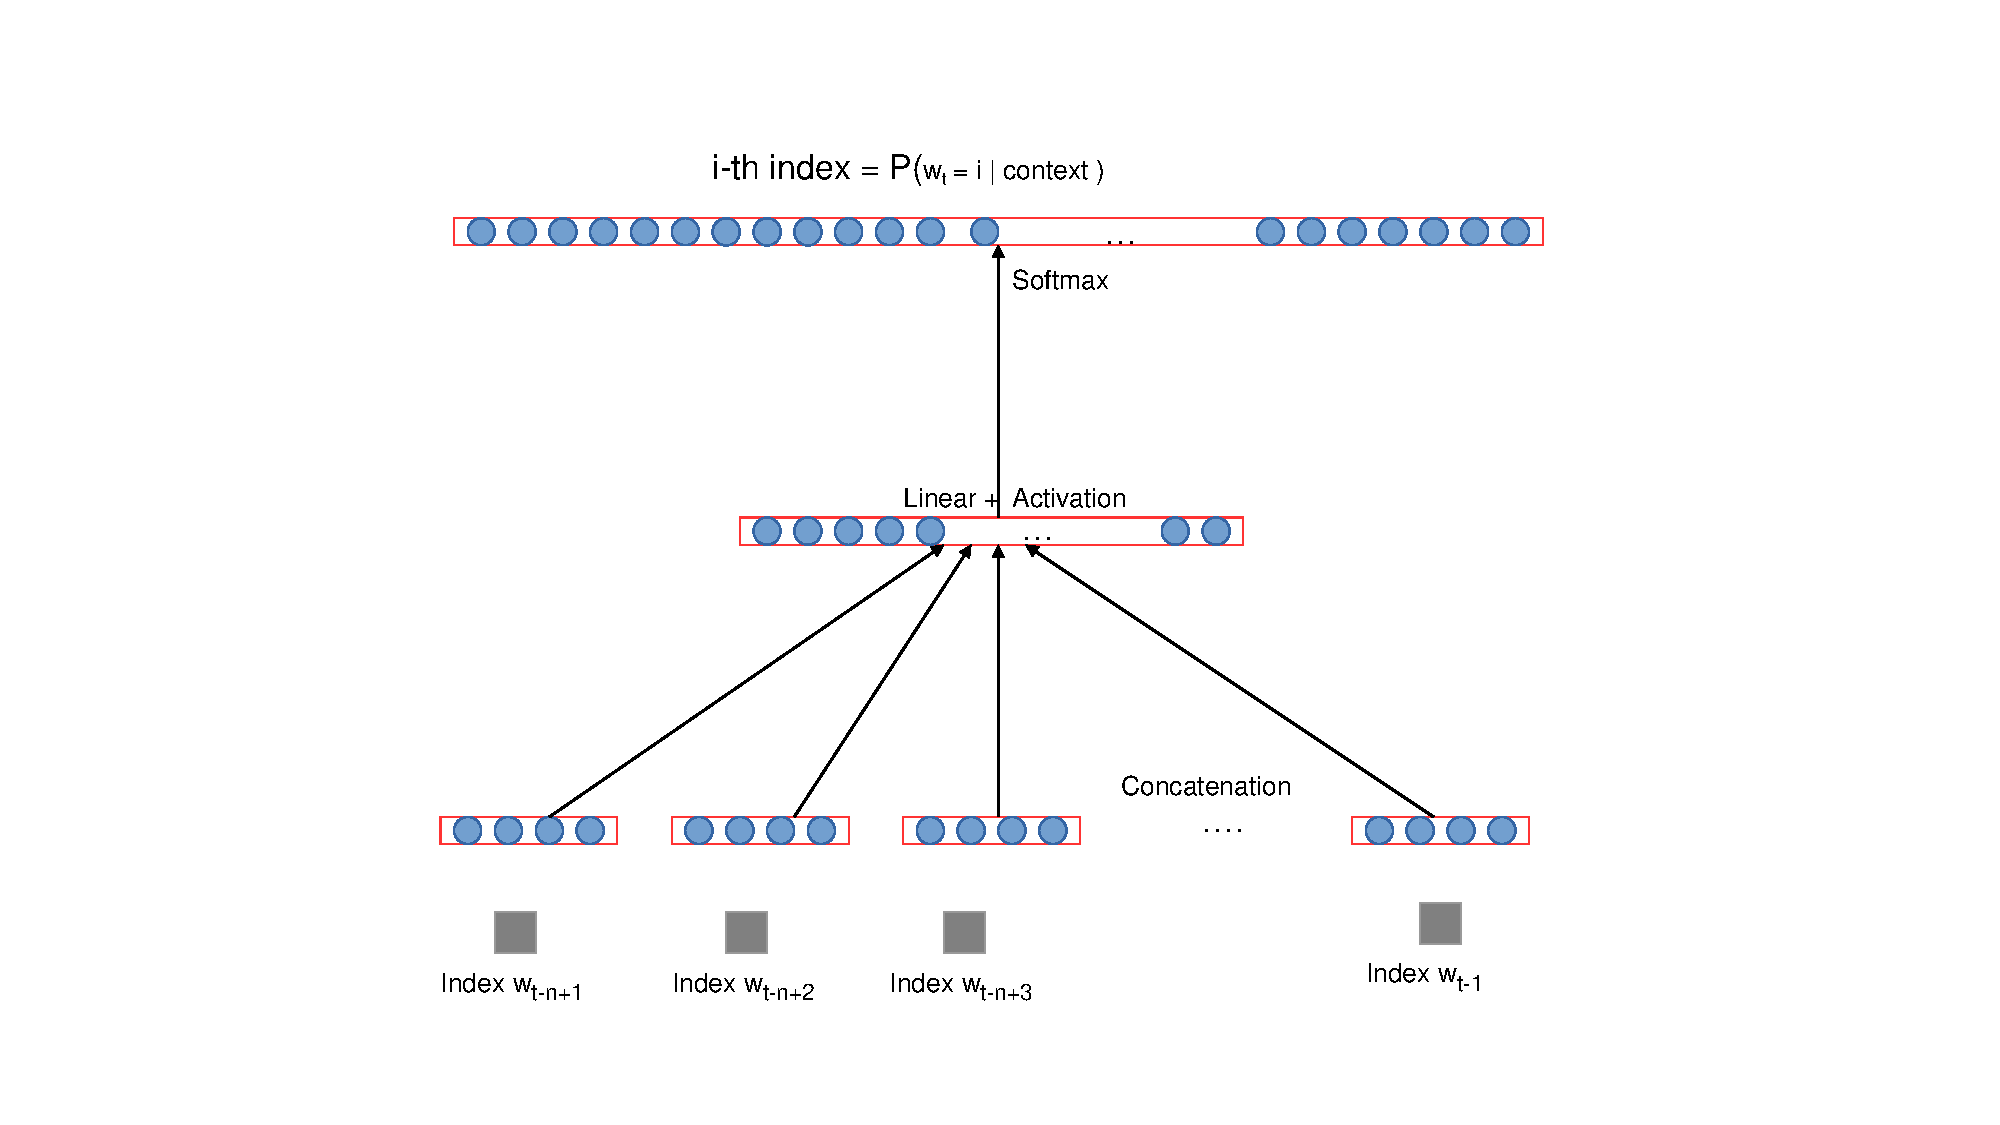
\includegraphics[width=\columnwidth]{figures/neuralLM.pdf}
~ \caption{Neural Language Model by Bengio et al~\cite{bengio2003neural}.}  
~ \label{fig:neuralBengio}
~ \end{figure}

\paragraph{Input layer}
The input layer constructs the embeddings of the words in the context, by using a shared word space and mapping each word in the context to a real-valued vector. Concretely, each word $w_i$ is represented as an 1-of-V coding, which is a long vector with the size of vocabulary V with all zeros except for the element corresponding to the word's index in the dictionary. Using this form of sparse coding, the word space (also called projection matrix $R$) is a matrix that contains V rows and each word embedding $v_i$ corresponds to one row of the matrix. The number of columns of the matrix is the size of the embedding, which is a tunable hyper-parameter. Notably, the values of the word vectors do not depend on the position of the word in the context. The context vector $i$ is the concatenation of the word vectors.

\begin{equation}
\begin{aligned}
i = \{R^T v_1; R^T v_2; .... ; R^T v_{n-1} \}
\end{aligned}  
\end{equation}


\paragraph{Hidden layer}
In the hidden layer, the input (context vector) is transformed nonlinearly, where each layer activation values are defined by

\begin{equation}
\begin{aligned}
h^j_{out} = f(W^j h_{in} + b^j) \\
h^1_{in} = i
\label{eq:hidden1}
\end{aligned}  
\end{equation}

In equation~\ref{eq:hidden1}, each hidden layer $h^j$ has the corresponding weights $W^j$ and $b^j$. The input of the first hidden layer is the context vector produced from the input (projection) layer. The size of the subsequent hidden layers are tunable hyper parameters. $f$ denotes a nonlinear activation function. Popular choices for the activation function are Tangent Hyperbolic, Sigmoid or ReLU, expressed in equation~\ref{eq:activation}. 


\begin{equation}
\begin{aligned}
 f(x) = 
	\begin{cases}
	\frac{\exp (x) - \exp (-x)}{\exp (x) + \exp (-x)}    \text{    if } f = \text{Tanh} \\
	\frac{1}{1 + \exp(-x)}                \text{     if } f = \text{Sigmoid} \\
	\max(0, x) \text{     if } f = \text{ReLU} \\
	\end{cases}
\label{eq:activation}
\end{aligned}
\end{equation}

\paragraph{Output layer}
The final layer of the network produces the probability distribution for all words in the vocabulary, thus having totally V nodes. Each neuron in the layer is associated to the probability of one word, as shown in Figure~\ref{fig:neuralBengio}. First, a linear transformation is used to obtain the unnormalised distribution:

\begin{equation}
\begin{aligned}
o = W^o h + b^o
\label{eq:linearoutput}
\end{aligned}  
\end{equation}

Notably, the values of $o$ is unnormalised because each element in o is associate to the score of each output word given the context vector. $W^o$ and $b^o$ are the corresponding weights and biases of the layer. Importantly, $W^o$ has the same form as the projection matrix at the input layer, since it also learns embedding for each word in the output vocabulary. Subsequently, the true probability distribution is estimated thanks to the~\textit{softmax} function:

\begin{equation}
p(w_i | h) = \frac{\exp(o_i)}{\sum_j \exp(o_j)}
\label{eq:softmax}
\end{equation}

In equation~\ref{eq:softmax}, the probability of each word $w_i$ given the encoded context $h$ is estimated by normalizing all values in $o$. Overall, the main tunable hyper-parameters of the network are the order of $n$-grams (the number of words in the context, which can range from 6 to 15), the sizes of hidden layers, and the word embedding size. The free parameters~$\Theta$ that are algorithmically learned from the data includes the projection matrix $R$, the weight matrices $W^h$ at the hidden layers, $W^o$ at the output layer and the biases $b^h$, $b^o$. 


\subsection{Training method}
From the machine learning perspective, the neural network language model has transformed the statistcal language modeling problem from a generative learning process to a discriminative classification problem. The free parameters of the network are trained by minimising the objective function, which is the log-likelihood~$\mathcal{L}$ of the  parameters~$\Theta$ given the training samples. The parameters are updated after each iteration based on some optimization techniques, among which Stochastic Gradient Descent (SGD) is most commonly used in neural language models \cite{zaremba2014recurrent,le2011structured,mikolov2010recurrent}. SGD and other variants such as Adadelta~\cite{zeiler2012adadelta} or RMSProp~\cite{tieleman2012lecture} require the computation of the first order derivatives of the loss function with respected to the parameters, which can be performed efficiently with the back-propagation algorithm~\cite{le1990handwritten}.

\subsection{Optimisation Process}
In this section, we describe the back-propagation flow in the standard feed forward neural language model - the core of the optimisation process. Back-propagation~\cite{rumelhart1985learning} involves using a dynamic programming strategy to compute the derivatives of the loss function with respect to the parameters layer by layer, based on the chain rules. In the standard network, the error derivatives are back-propagated from the output layer to the input (projection) layer.

\paragraph{Objective Function}

The smoothing function that we approximate with the neural network has parameters that can be iteratively tuned in order to~\textbf{maximise the log-likelihood of the training data}. 

The network aims at maximising the probability of the label word given the context, hence the objective function is typically chosen as the Negative Log-Likelihood function. Assuming we have N samples, each of which is an $n$-gram, we can compute the loss function over the training data as follows:

\begin{equation}
\mathcal{L} = - 	\sum_{i}^N \ln P( w_i | w_{i-n+1}^{i-1} ) \\
\label{eq:objective}
\end{equation}

The objective function is in line with the perplexity that we want to minimise (which is equivalent with maximising the log-likelihood of the training data). For ease of understanding, we denote the derivative of the loss function~$\mathcal{L}$ at~\textit{each} sample or batch of samples with respect to a variable $x \in \Theta$ by $dx$.  

For each sample, let's $w$ be the index of the predicted word $w_i$ in the vocabulary, we have:

\begin{equation}
\begin{aligned}
- \log P(w_i |  w_{i-n+1}^{i-1})  = - \log P(w | h) \\
= - log (\frac{\exp (o_w)}{\sum_i exp(o_i)}) \\
=  log(\sum_i \exp(o_i)) - o_w
\label{eq:objective2}
\end{aligned}
\end{equation}

Subsequently, we compute the error derivatives $dx$ given the parameters in each layer using back-propagation:

\paragraph{Output layer}

The derivatives at the output layer:

\begin{equation}
do_i = 
\begin{cases}
1 - p_i \text{ if } i == w \\
-p_i \text{     otherwise}
\end{cases}
\end{equation}

Notably, $o_i$ denotes the $i^{th}$ element of the vector $o$, which is the unnormalised distribution of the vocabulary given the encoded context $h$. 

\paragraph{Hidden layers}
As a result, we can compute the derivatives with respect to the parameters and the previous hidden layer $h$, based on the original inference from Equation~\ref{eq:linearoutput}. 

\begin{equation}
\begin{aligned}
dW^o = doh^T \\
db^o = do \\ 
dh = {W^o}^Tdo \\
\end{aligned}
\end{equation}


For the inner hidden layers, the  derivatives for the linear components are computed similarly, by replacing $do$ with $dh$ (the output of the previous hidden layer is the input of the next hidden layer). However, we have to take into account the non-linear activation functions, which are shown in the inference equation for the previous hidden layers:

\begin{equation}
h_{next} = f(W^h h_{prev} + b^h)
\end{equation}

With $W^h$ and $b^h$ are the corresponding weights connecting $h_prev$ to $h_next$. The derivatives are computed as follows:

\begin{equation}
\begin{aligned}
d[W^h h_{prev} + b^h] = f'(h_{next}) dh_{next} \\
db^h = d[W^h h_{prev} + b^h] \\
dW^h = d[W^h h_{prev} + b^h]h_{prev}^T \\
dh_{prev} = {W^h}^T d[W^h h_{prev} + b^h]
\label{eq:dhidden}
\end{aligned} 
\end{equation}

The derivative function of $f$, $f'$:

\begin{equation}
\begin{aligned}
f(x) = 
\begin{cases}
1 - \text{Tanh}(x)^2   \text{    if } f = \text{Tanh} \\
\text{Sigmoid}(x) - \text{Sigmoid}(x)^2                \text{     if } f = \text{Sigmoid} \\
1 \text{ when } x > 0 \text{ and 0 otherwise}  \text{     if } f = \text{ReLU} \\
\end{cases}
\label{eq:dactivation}
\end{aligned}
\end{equation}


\paragraph{Input Layer}

The derivative function of the input layer is identical to Equation~\ref{eq:dhidden} and Equation~\ref{eq:dactivation}, considering that the input layer is the layer before the first hidden layer. 

\paragraph{Parameter Update}

After obtaining the derivatives of the loss function with respect to all parameters in the network, we can update the parameters following Stochastic Gradient Descent. The method is based on the phenomenon that the gradient of a function always points towards the direction of maximal increase at any point. The update rule is as follows with the learning rate parameter $\alpha > 0$:

\begin{equation}
x = x - \alpha dx
\label{eq:sgd}
\end{equation}

The learning rate is also considered as a function of the number of samples trained in the data. Typically, the learning rate is updated after the model observes a number of training examples, with two most common ways. The first way is to exponentially decrease the learning rate after some training samples with a~\textit{learning rate decay}, normally an epoch (training all samples in the training data). The second way is to reduce the learning rate based on a validation data. After each epoch, if the perplexity on the validation data is decreased, the learning rate is kept the same, otherwise it is multiplied by the learning rate decay.


\subsection{Recurrent Neural Language Models}

Compared to the statistical $n$-gram models, the feed-forward neural language models had created a considerable leap in representation by combining distributed representation of words with a robust classifier to generalise from observed sequences. As can be seen from various works~\cite{schwenk2007continuous,le2011structured}, the feed-forward language model significantly outperformed the traditional Knesey-Ney back-off models. However, the feed-forward models require a fixed input size, thus still rely on the Markov Assumption which limits the context to a particular number of words, even when the context size can be huge up to $10$. In order to model long sentences, or even paragraphs with long-term dependencies, it is beneficial to investigate in models that can be flexible in terms of input size. For example, if the distance between the open bracket and the closed counterpart is further than the $n$-gram input size, the feed forward model may forget to close the brackets after seeing the initial one. Ideally, as the learning process of human is associated with a memory that keeps the current information (such as topics), similar structure should be simulated and integrated in the network.

\paragraph{Recurrent Neural Networks} RNN~\cite{elman1990finding} are a class of neural networks that can efficiently model sequences by using a dynamic memory structure. While the feed-forward network can only receive one input and compute the corresponding output without any relation with other inputs, the recurrent counterpart takes the input as a~\textit{series of time step}  $x_1, x_2, \dots, x_n$ and processes them one by one, taking into account the information stored in the previous steps. Concretely, for each input $x_i$, the network updates the hidden memory $h_i$ based on the previous one $h_{i-1}$. 

%The ''Vanilla`` model~\cite{elman1990finding} uses a simple combination of the input and the previous memory:

\begin{equation}
h_i = \mathcal{F}(x_i, h{i-1})
\end{equation}

 We will cover some popular RNN variations in the upcoming sections. In general, the strong point of these models lie in the ability to dynamically model sequences with arbitrary length, which the feed-forward neural networks cannot achieve. The advantage comes with the cost that the recurrent models are generally hard to train, due to the properties of back-propagation. A change in an arbitrary position of the sequence can lead to a change in the objective function, therefore training methods for RNNs typically have to trace back the previous time steps. In other words, the RNNs are equivalent to feed-forward neural networks with many hidden layers that share parameters across each other. Importantly, the model capacity of RNNs do not depend on the length of the sequences, but in the recurrence mechanism - the way the hidden layers are updated. 
 
\paragraph{Recurrent Language Models} Language Modeling can be viewed as a sequence modeling problem, in which each time step corresponds to one word. The first recurrent language model (RNNLM)~\cite{mikolov2010recurrent} employed the ``Vanilla'' model of Elman et al~\cite{elman1990finding} as can be seen in Figure~\ref{fig:SimpleRNN}, in which the hidden steps are updated as follows:

~ \begin{figure}[!t]
	~ \centering
	~ 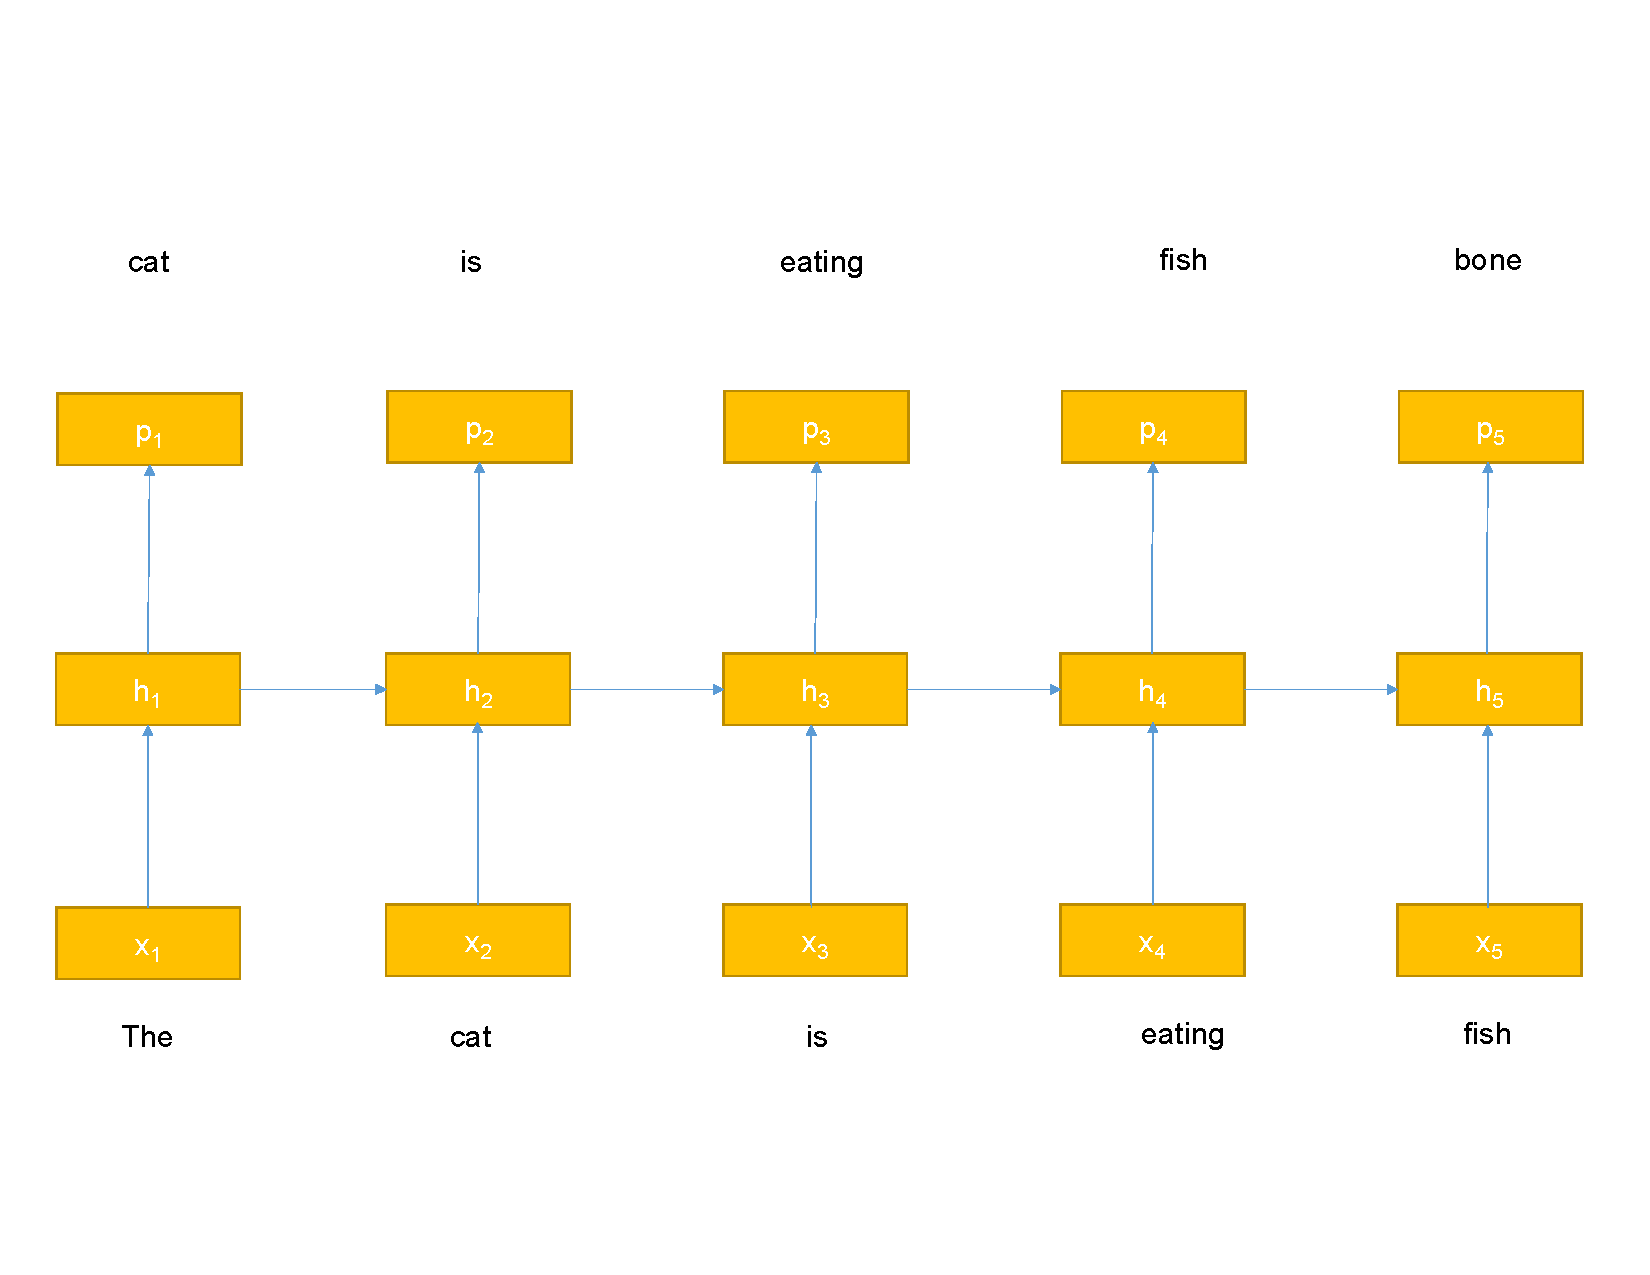
\includegraphics[width=\columnwidth]{figures/rnn.pdf}
	~ \caption{A simple RNNLM~\cite{mikolov2010recurrent} predicting the sequence ``The cat is eating fish bone''.}  
	~ \label{fig:SimpleRNN}
	~ \end{figure}


\begin{equation}
h_i = f(Wx_i +  Uh{i-1} + b)
\end{equation}

The activation function $f$ can be either Tangent Hyperbolic, Sigmoid or ReLU as mentioned before. The starting state $h_0$ is set to 0 to denote the initial state of the memory. In each time step, the RNNLM can optionally produces the probability distribution for a predicted word, given the sequence that network has scanned previously. The probability distribution over the vocabulary is derived similarly to the feed-forward networks:

\begin{equation}
\begin{aligned}
o_i = W^oh_i + b^o \\
p_i = \text{softmax}(o_i)
\end{aligned}
\end{equation}

with the Softmax function explained in Equation~\ref{eq:softmax}. To be clear, $o_i$ and $p_i$ denote the unnormalised and normalised distribution generated at time step $i$. For the language modeling scenario, the input and output samples of the network in each training iteration are two sequences $X \text{ and } Y$ in which the output sequence is the shift-by-1 version of the input sequence. The parameter set of the network including $W, b, U, W^o \text{ and } b^o$ are shared across time steps. 


\subsubsection{Training Recurrent Networks}

Similarly to the feed-forward models, The recurrent models can also be efficiently trained with stochastic gradient descent (SGD). However, since the networks contain shared parameters at arbitrary numbers of time steps, the gradients are computed differently using back-propagation through time (BPTT). The details of this algorithm are divided into two parts: the local gradients computed  at each time step, and the global gradients accumulated by un-folding the networks. 

\paragraph{At each time step}

% How to compute the gradients

\paragraph{For global derivatives}

Backpropagation through time algorithm 

\paragraph{Problems with BPTT}

Although truncated back-propagation through time provides a practical training method for RNNs, the nonlinear iterative nature of the simple RNN architecture still makes capturing long-term dependencies difficult. The two common problems encountered while training RNNs are the~\textit{exploding} and the~\textit{vanishing} gradients~\cite{bengio1994learning,pascanu2013difficulty}. On the one hand, the gradients can be exponentially large as in the back-propagation through time process which is detrimental for learning. One the other hand, we can also experience the phenomenon that gradients go quickly towards zero after being propagated through time steps. Consequently, the model is not able to track the signal and complete loses the memory trace in the past. For example, the original RNNLM normally has to truncate the BPTT at about $5-10$ steps, which has the same modeling capacity and performance with $10$-gram feed-forward models~\cite{mikolov2011extensions,hai2012measuring}. The gradient exploding problem can be tackled adequately using gradient clipping. Pascanu et al~\cite{pascanu2013difficulty} suggested to clip the norm of the gradients (for all parameters): given a gradient vector $dx$ that is computed with BPTT, if the norm $||dx||$ is greater than a threshold value $\delta$, then $dx$ would be softly scaled:

\begin{equation}
dx \leftarrow dx\frac{||dx||}{\delta}
\end{equation}

%Explain mathematically
\paragraph{Dealing with gradient vanishing}

A number of solutions were proposed to solve the gradient vanishing problem. We will make a brief review of the most prominent approaches. First, Mikolov et al~\cite{mikolov2014learning} proposed to integrate another memory layer which is formed by the bag-of-word addition of the input words over time, decays slower than the main hidden memory and is initialised as an identity matrix. The same initialisation trick is applied together with using Rectified Linear Units (ReLU) as the activation function in~\cite{le2015simple}. While both works mentioned are fairly simple, the RNNs can also be trained efficiently with second order derivatives using Hessian-Free optimization~\cite{martens2011learning}. Even though the method was prove to allow the network to acquire a reliable memory which can remain stable after hundreds of time steps, it is not easy to implement efficiently compared to traditional back-propagation. The most successful method that is applied to sequential modeling in general and language modeling in particular is the Long-Short Term Memory LSTM networks~\cite{hochreiter1997long} that use an explicit memory cell combined with a gating mechanism to intensively deal with the gradient vanishing problem.

\paragraph{LSTM Structure} The intuition of an LSTM starts from the integration of a linear memory unit, so that the gradient can flow smoothly during the back-propagation through time steps using a memory cell $c_t$. 

\begin{equation}
c_t = c_{t-1} + f(Wx_i +  Uh{i-1} + b)
h_t = c_t
\end{equation}

This approach is referred as ``Leaky integration units''~\cite{bengio2013advances}. In the BPTT process, the gradient can flow over exactly one path through the memory units $c_i$, and since $dc_i = dc_{i-1}$, the gradients are guaranteed to not vanish. The recurrent architecture should also be able to be adequately robust to train long sequences, where there are certain inputs which are irrelevant to the modeling task. Sometimes, the memory of the network should be refreshed, for example at the beginning of a new utterance in Speech Recognition~\cite{graves2005framewise} or a new sentence in Machine Translation~{sutskever2014sequence}. Hochreiter et al~\cite{hochreiter1997long} enhanced the architecture by adding flexible and trainable gates that allows the RNN to reset the memory, control the amount of input and output respectively. The adaptive gates are built from the current input $x_t$ and the previous hidden memory $h_t$. 

The gates of the network include: the forget gate $f_t$ is used to directly control the memory flow $c_t$ to cut the connection with the previous steps, the input gate $i_t$ decides the amount of input to be incorporated, the output gate $o_t$ controls the amount of memory flow to be produced for the task and finally the candidate memory unit $\tilde{C}$ that contributes to the current memory flow. All gates are defined similarly, with the first three gates use the Sigmoid activation to force the values to be in \{0, 1\}, while the candidate memory uses the Tanh activation function.

\begin{equation}
\begin{aligned}
f_t = \text{Sigmoid}(W_fx_t + U_fh_t + b_f) \\
i_t = \text{Sigmoid}(W_ix_t + U_ih_t + b_i) \\
o_t = \text{Sigmoid}(W_ox_t + U_oh_t + b_o) \\
\tilde{C}_t = \text{Sigmoid}(W_cx_t + U_ch_t + b_c) \\
\end{aligned}
\label{eq:lstm1}
\end{equation}

In the next step, we decide the new information to be stored in the new memory cell. The cell is updated by combine the input gate and the candidate memory unit. Also, the forget gate is employed to drop certain information from the previous memory cell. Consequently, we come up with a new memory cell as follows:

\begin{equation}
C_t = f_t * C{t-1} + i_t * \tilde{C}_t
\label{eq:lstm2}
\end{equation}

Finally, we update the hidden state with the new cell state and the output gate:

\begin{equation}
h_t = o_t * \text{Tanh}(C_t)
\label{eq:lstm3}
\end{equation}

In Equations~\ref{eq:lstm2} and~\ref{eq:lstm3}, the symbol $*$ denotes element wise matrix multiplication. The implementation of LSTM can be efficient by computing all gates in one single matrix multiplication, then applying the activation functions on different parts of the output. In practice, one can experience different implementation variations of LSTMs and RNNs in terms of initialisation, bias usage or different gate implementations such as the Gated Recurrent Unit~\cite{cho2014learning}. The empirical research of~\cite{zaremba2015empirical} shows that there is not any substantial difference in terms of performance between different LSTM variations. 

\paragraph{Training LSTM}

Rewrite the Backpropagation through time from RNN
%
%\section{Analysis}
%
%
%\subsection{Computational Complexity}
%
%\textbf{Bottleneck in the Softmax layer}
%
%\textbf{Approximating the Softmax}

%\section{Analysis}
%
%The most important achievement of neural network language models is the ability to model word representations with low dimension embeddings that can capture syntactic and semantic properties of words~\cite{mikolov2013distributed,mikolov2013efficient}. Such ability is trained simultaneously with the classifier in order to capture linguistic regularities, which helps the network to generalise over observed sequences. 
%
%Despite the fact that the state-of-the-art language models consist of a shared projection space between words, they still treat the context as a sequence of discrete symbols. The feed-forward network simply concatenate the word vectors and learn the non-linear mapping functions to get word combinations, while the recurrent models take one word as a time step, whose weakness is that a particular time step does not have any information about future steps. In fact, it is useful to take into account the collocations and multi-word expressions in the context. For example, the English word ``get'' can acquire different meanings when paired with different propositions, which the word embeddings hardly can represent. 
%
%Such word combinations are often identified by statistical methods~\cite{sag2002multiword}, which requires an intensive scanning through the data to find frequent combinations. In the context of the neural networks, it is intuitive to use a special neural network layer that has the~\textit{convolution} property, which goes through the input sequence by scanning with a small window to find pattern features. 





%\chapter{Neural Network Language Models}
%\label{c:nnlm}

\chapter{Convolutional Neural Language Models}
\label{c:cnn}
\section{Related works}

Convolutional Neural Networks (CNNs) were originally designed to deal
with hierarchical representation in Computer
Vision~\cite{lecun1995convolutional}. Deep convolutional networks have
been successfully applied in image classification and
understanding~\cite{karen2014vgg,kaiming2015resnet}. In such systems
the convolutional kernels learn to detect visual features at both
local and more abstract levels.

In NLP, CNNs have been mainly applied to static classification task 
for discovering latent structures in text. \newcite{kim2014sentence} use a
CNN to tackle sentence classification, with competitive results. This
work also introduces kernels with varying window sizes to learn
complementary features at different aggregation
levels. \newcite{Kalchbrenner2014conv} propose a convolutional
architecture for sentence representation that vertically stacks
multiple convolution layers, each of which can learn independent
convolution kernels. CNNs with similar structures have also been
applied to other classification tasks, such as semantic
matching~\cite{hu2014convolutional},
%\gbt{what is semantic matching? we call it sentence matching in the intro}
relation extraction~\cite{nguyen2015relation} and information
retrieval~\cite{shen2014latent}.  In
contrast,~\newcite{collobert2011natural} explore a CNN architecture to
solve various sequential and non-sequential NLP tasks such as
part-of-speech tagging, named entity recognition and also language
modeling. This is perhaps the work that is closest to ours in the
existing literature. However, their model differs from ours in that it
uses a max-pooling layer that picks the most activated feature across
time, thus ignoring temporal information, whereas we explicitly avoid
doing so. More importantly, the language models trained in this work are only
evaluated through downstream tasks and through the quality of the
learned word embeddings, but not on the sequence prediction task
itself.

In this work we focus on statistical language modeling, which differs
from most of the tasks where CNNs have been applied before in multiple ways. First,
the input normally consists of incomplete sequences of words rather
than complete sentences. Second, as a classification problem, it
features an extremely large number of classes (the words in a large
vocabulary). Finally, temporal information, which can be safely
discarded in many settings with little impact in performance, is
critical here: An $n$-gram appearing close to the predicted word may
be more informative, or yield different information, than the same
$n$-gram appearing several tokens earlier.
%A crucial difference between the aforementioned problems and language modeling is that 
%the context in each language modeling sample is normally not a full sentence. This property, together with temporal dependencies, makes 
%language modeling the more difficult task. 

%~ CNNs have also been applied directly on one-hot word vectors rather
%~ than word embeddings~\cite{johnson2015semi,johnson2015semi} in order
%~ to reduce the number of free parameters or over character
%~ embeddings~\cite{zhang2015text,yoon2015character}.
%In~\cite{zhang2015text}, the CNNs can operate on top of character sequences for classification. With the same approach,~\cite{yoon2015character} use time-delayed networks for word representation based on characters for better morphological discrimination. 

%The traits of our work are similar with Tag prediction from Twitter~\cite{weston2014tagspace}{\bf How?}. Besides, the memory network~\cite{sukhbaatar2015end} also shared some mechanical similarity with the convolutional networks, in which the context is scanned by the model multiple times for prediction{\bf Is this relevant?}. In~\cite{wang2015gen}, the author proposed a convolutional structure that can process contexts at any size, but the comparison between their model and the recurrent network is unclear, as well as their result is outperformed by our solid feed-forward baseline{\bf How does their model differ from ours?}.





\section{Base FFLM}

Our CNN is constructed by extending a feed-forward language model (FFLM) with convolutional layers. In what follows, we first explain the implementation of the base FFLM and next, we describe the CNN that we study.

%~ Our baseline feed-forward language model (FFLM) is based on that of
%~ \newcite{bengio2006neural}, with a few modifications that much improve
%~ performance. The model is illustrated in Figure~\ref{fig:baseline} and
%~ works as follows. First, the input tokens are passed through a
%~ projection layer that fetches their associated vectors from a lookup
%~ table and concatenates them all together. This large vector is then
%~ fed to a fully-connected layer to produce a hidden layer. Next, and
%~ differently from the original model, a highway layer is
%~ used~\cite{srivastava2015highway}. 

Our baseline feed-forward language model (FFLM) is almost identical to the original model proposed by  ~\newcite{bengio2006neural}, with only slight changes to push its performance as high as we can, producing a very strong baseline. In particular, we extend it with highway layers and use Dropout as regularization. The model is illustrated in Figure~\ref{fig:baseline} and works as follows. First, each word in the input $n$-gram is mapped to a low-dimensional vector (viz. embedding) though a shared lookup table. Next, these word vectors are concatenated and fed to a highway layer ~\cite{srivastava2015highway}.
%The mechanism of highway layers is we can combine the non-linear affine transformation of an input layer with itself to create the output hidden layer. 
%Assuming the input and output of the highway layer is $H_I$ and $H_O$. The materials for a highway layer is a typical non-linear transformation $H$ and a transform gate $T$
%\begin{equation}
%\begin{aligned}
%H = f(H_I . W_h + b_h) \\
%T = (H_I . W_t + b_t)
%\end{aligned}  
%\end{equation}
%$W_h, b_h$ and $W_t, b_t$ are linear connected weights for the model, $f$ is a nonlinear function (ReLU in our work). Notably, the highway layer requires double the weights than a typical linear connected layer.
%The output of the highway layer is the combination of the transformed input and a part of the input carried away to the output. 
%\begin{equation}
% H_O = H \ast T + H_I \ast (1 - T)
%\end{equation}
Succinctly, highway layers improve the gradient flow of the network by computing as output a convex combination between its input (called the \emph{carry}) and a traditional non-linear transformation of it (called the \emph{transform}).
As a result, if there is a neuron whose gradient cannot flow through the transform component (e.g., because the activation is zero), it can still receive the back-propagation update signal through the carry gate.  %While deep feed-forward neural networks have not been shown to yield an important comparative advantage with respect to more shallow models~\cite{arisoy2012deep} ,
 We empirically observed the usage of a single highway layer to improve importantly the performance of the model. Even though a systematic evaluation for this model is beyond the scope of the current paper, our empirical results demonstrate that it is a very competitive one (see Section \ref{sect:exp}).    

%~ fed to a fully-connected layer to produce a hidden layer 
%~ works as follows
Finally, a softmax layer computes the model prediction for the upcoming word. We use ReLU for all non-linear activations and Dropout~\cite{hinton2012dropout} is applied between each hidden layer.%, which increase the regularisation capability of the network by randomly preventing forward activation of neurons during training. Notably, dropout is only applied to the fully connected components, thus having no effect on the convolutional layer .After the hidden layers, the output layer of the network is a softmax over the entire vocabulary. In experiments with large vocabularies, we factor the softmax layer with a hierarchical softmax~\cite{mikolov2011extensions} in order to improve the speed of the network. Specifically, the words are clustered into classes based on the unigram distribution frequency. After that, the network estimates the probability distribution over the class and another distribution over the words in that particular class. As a result, we can avoid large matrix computation. Finally, the activation function used in all experiments is ReLU. Not only can ReLU avoid gradient saturation, the activated neurons always have positive values, this facilitating the analysis of subsequent hidden layers




%~ Highway layers are
%~ $\dots$. \textbf{and Dropout? and Batch-norm?}. \textbf{Did we use HSM
  %~ for the experiments or not?} \gbt{Agree, we need info about
  %~ that}. Finally, a softmax layer yields the output of the network.

%~ \gbt{VERY IMPORTANT: Enlarge the font in all the figures (it should be approx.\ as large as
  %~ the one in the text). Add ``Hidden layer'' or simply ``H'' to the graph so
  %~ you can reference it in the text. What does the layer between the
  %~ highway layer and the softmax do?}

%~ \gbt{thanks for enlarging the font of the baseline model figure;
  %~ please enhance the font of figures 2 and 3, too}

%This section describes the general structure of our baseline model, which is illustrated in Figure~\ref{fig:baseline}. Essentially, we use the original architecture proposed in~\cite{bengio2006neural}. In the first layer, a lookup table is used to store the shared embedding space and query the context word vectors, which are in turn concatenate into one single context vector. The output layer is a softmax over the whole vocabulary, which can be factorized into an hierarchical softmax to reduce the complexity of the model~\cite{le2011structured,mikolov2011extensions}. Regarding the hidden layers, multiple hidden layers seem to have optimization problems~\cite{arisoy2012deep}. We empirically optimized the baseline network by using an additional highway layer~\cite{srivastava2015highway}, thus making the network similar to the lateral network in~\cite{devlin2015pre}. Furthermore, we use dropout~\cite{hinton2012dropout} to enhance regularisation for the model. 

%\textbf{Fixme: move later to the experimental part} Regarding the context size, we use $16$ words in the context for most of our experiments. Neural network language models, by their nature, can scale up the distribution for an arbitrary context size, which could be too sparse for count-based models~\cite{kneser1995improved}. It is notable that, the feed forward models in~\cite{hai2012measuring} do not benefit much from a context larger than $10$, yet the author only took into account the words in the current sentence. 
% Compared to the original architecture, our baseline model yield a better performance, due to the above mentioned extensions and better optimization ({\bf really? we just use SGD}) and regularisation, as shown in section~\ref{sect:exp}.

~ \begin{figure}[!t]
~ \centering
~ 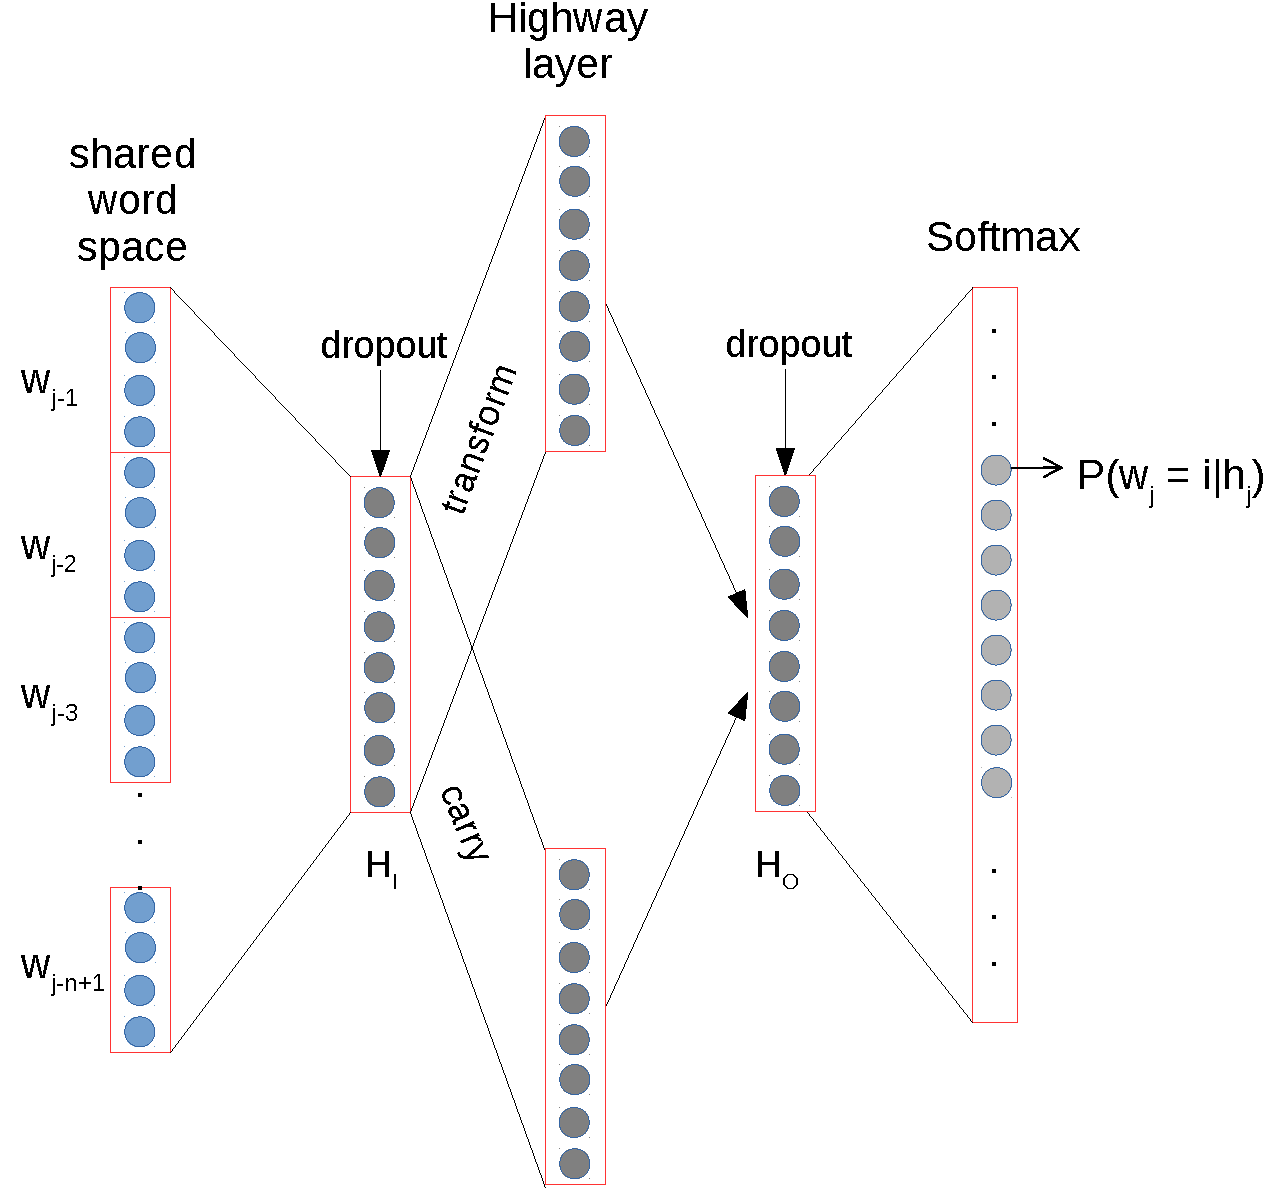
\includegraphics[width=\columnwidth]{figures/baseline.pdf}
~ \caption{Overview of baseline FFLM.}  
~ \label{fig:baseline}
~ \end{figure}
%\begin{figure*}[!t]
%\begin{minipage}{.5\linewidth}
%
%\centering
%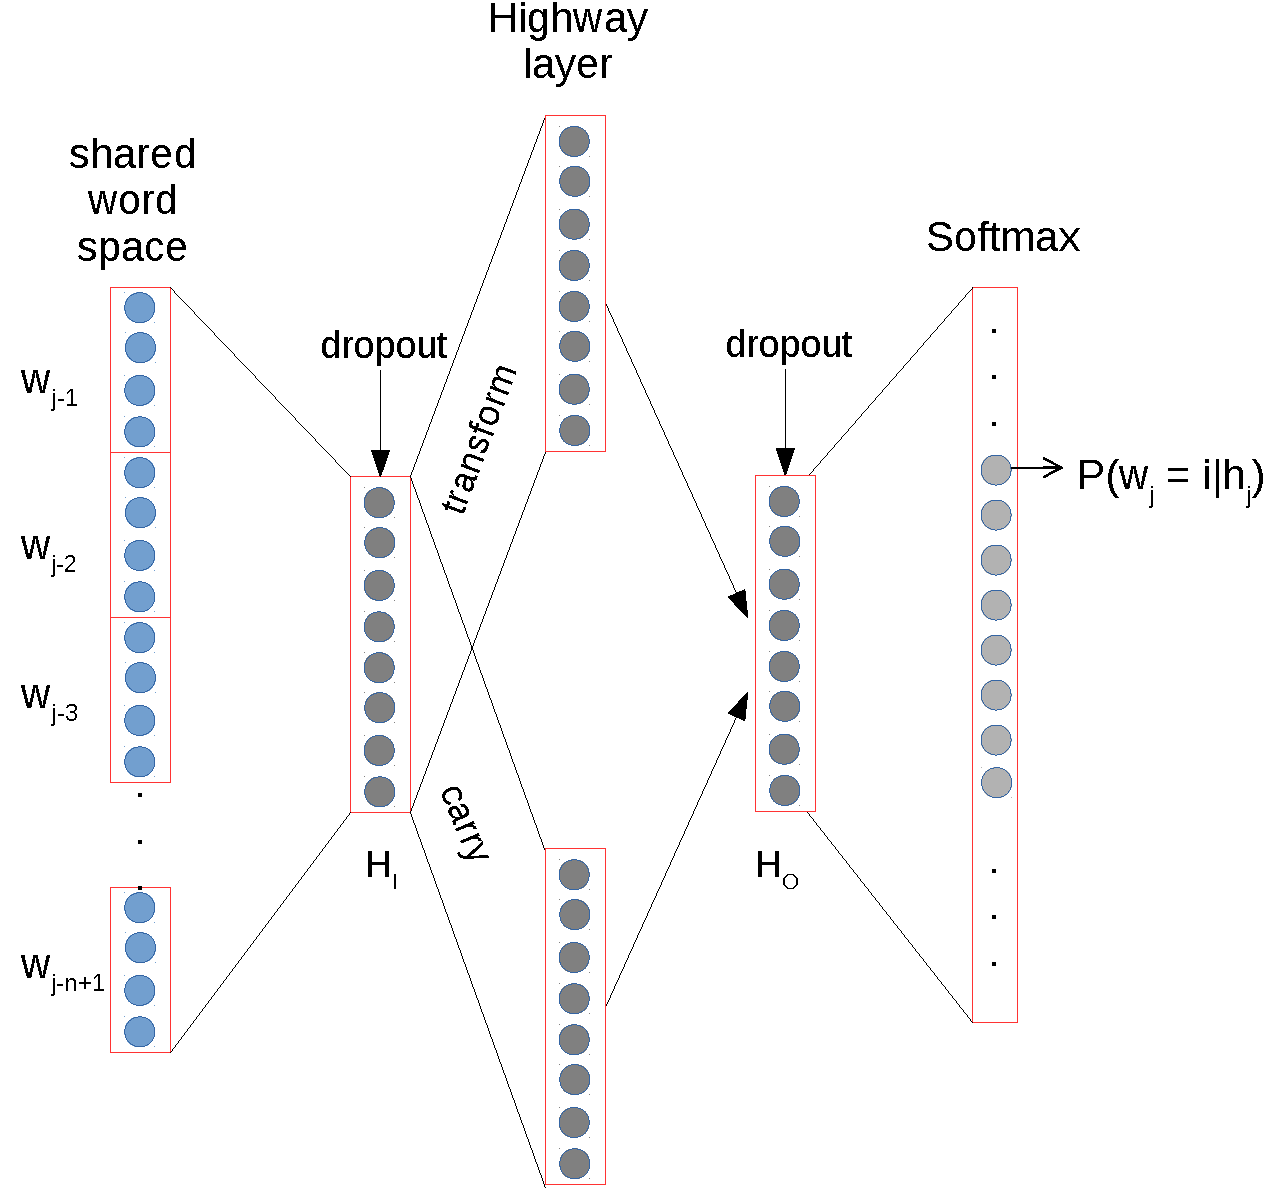
\includegraphics[width=1\linewidth]{figures/baseline.pdf}
%\caption{Overview of baseline FFLM.}  
%\label{fig:baseline}
%%~ \end{figure}
%\end{minipage}
%\begin{minipage}{.5\linewidth}
%%~ \begin{figure}[!t]
%\centering
%\vspace*{15mm}
%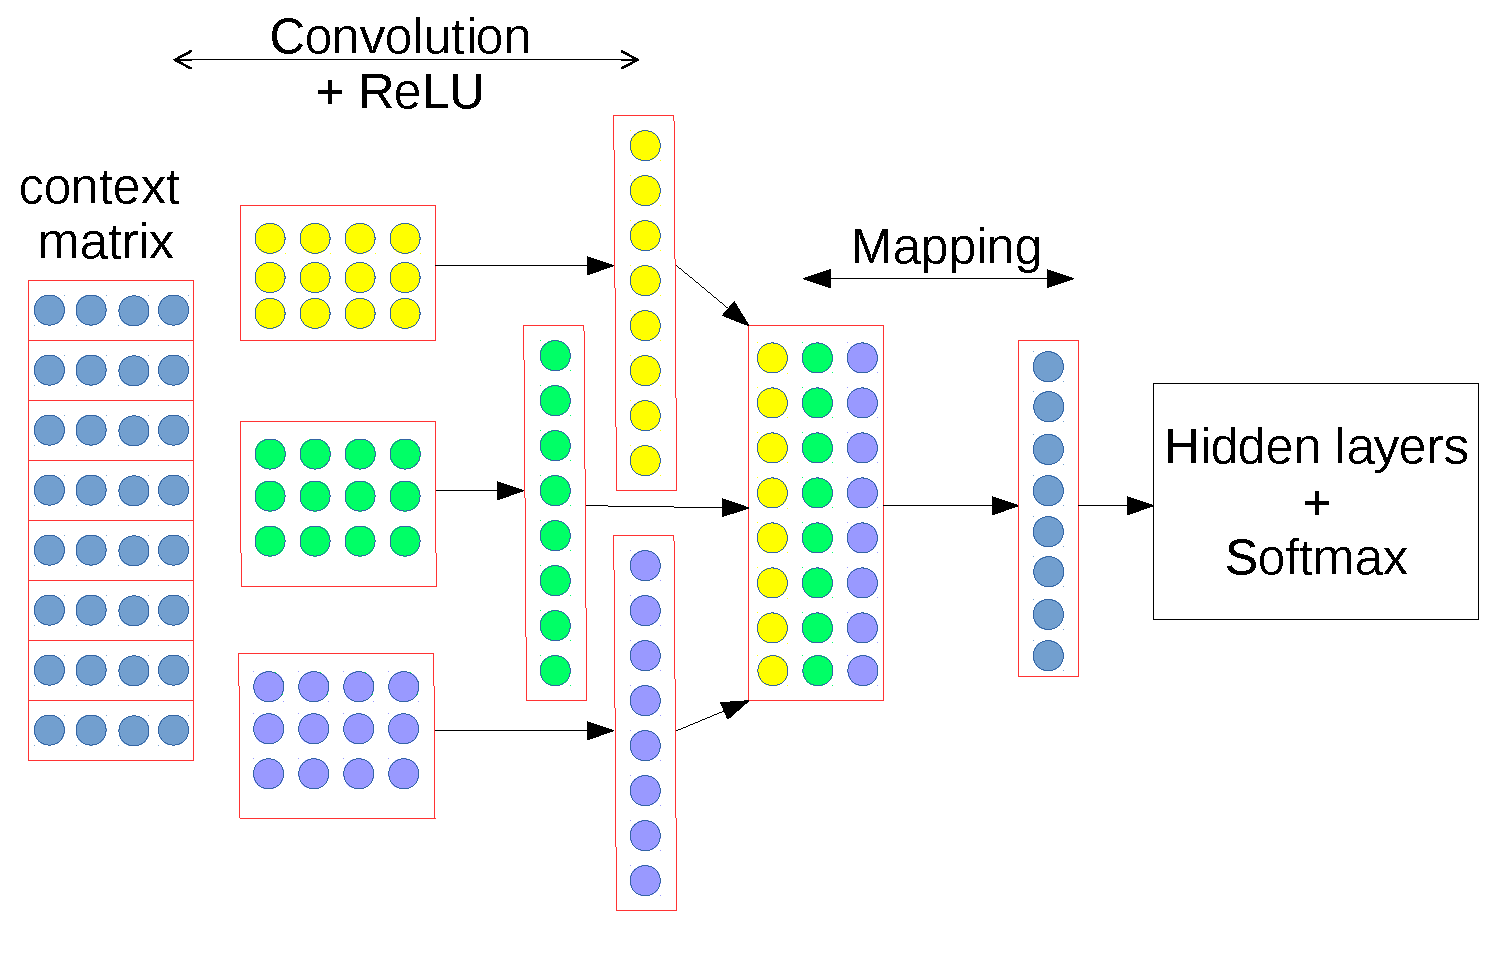
\includegraphics[width=1\linewidth]{figures/convolution.pdf}
%\vspace*{4mm}
%\caption{CNN layer on top of the context matrix.}  
%\label{fig:simpleconv}
%\end{minipage}
%\end{figure*}

\section{CNN and variants}

The proposed CNN network is produced by injecting a convolutional layer right after the words in the input are projected to their embeddings (Figure \ref{fig:simpleconv}). Rather than being concatenated into a long vector, the embeddings $x_i \in \mathbb{R}^k$ are concatenated transversally producing a matrix $x_{1:n}  \in \mathbb{R}^{n \times k}$, where $n$ is the size of the input and $k$ is the embedding size.  %Consequently, we minimally change the network structure and the number of parameters and the network only learns word patterns through the convolutional kernels.
%Similarly to \newcite{collobert2011natural} and
%\newcite{kim2014sentence}, we utilize a time-delayed
%network~\cite{waibel1989phoneme} where the input vectors are convolved
%through various learned kernels.
%
%The computation is done as follows. Let $x_i \in \mathbb{R}^k$ be the
%vector associated with the $i$-th input context word. First, all these
%vertical vectors are concatenated horizontally leading to a matrix
%$x_{1:n}$ of size $k \times n$:
%\begin{equation}
%x_{1:n} = x_1 \oplus x_2 \oplus \dots \oplus x_n
%\end{equation}
% In which, $x_{1:n}$ is a matrix of size $k \times n$, which is
% different to the long context vector in the baseline model.
This matrix is fed to a time-delayed layer, which convolves a
sliding window of $w$ input vectors centered on each word vector using a
parameter matrix $W \in \mathbb{R}^{w \times k}$. Convolution is performed
by taking the dot-product between the kernel matrix $W$ and each
sub-matrix $x_{i-w/2:i+w/2}$ resulting in a scalar value for each position $i$ in input context. This value represents how much the words encompassed by the window  match the feature represented by the filter $W$. A ReLU activation function is applied subsequently so negative activations are discarded. %In summary, we compute:
%\begin{equation}
%y_i = f(W \ast x_{i:i+w-1} + b)
%\end{equation}
%where $W$ and $b$ are learnable parameters of the convolutional
%kernel, and $f$ is a nonlinear function. A specific kernel can be %seen
%as a detector for a particular feature and the output $y_i$ can be
%seen as an indication for whether the feature is present or not at the
%current time step. 
This  operation is repeated multiple times using
various kernel matrices $W$,  learning different features independently. Here we tie the number of learned kernels to be the same as the embedding dimensionality $k$. Thus, the output of this stage will be another matrix of dimensions $n \times k$ containing the activations for each kernel at each time step.

%Typically, there are four main hyper-parameters involved in deciding
%the output sizes of the convolutional neural networks. The number of
%kernels indicates the {\bf depth} (number of features to be detected)
%of the output, while the {\bf kernel size}, the {\bf stride} (the distance
%between two convolutional steps), and {\bf zero paddings} at the beginning
%and the end of the input decides the number of convolutional steps.  In order to
%simplify the experiments, we assume that the number of convolutional
%features is proportional to the embedding dimensionality, and fix the
%number of kernels to be equal to the latter ($k$). The stride is kept
%to $1$ and zero padding is added with respect the the kernel width
%(number of words in one step). As a result, the size of the
%convolutional output is $n \times k$, which has the same neurons as
%the input embeddings. 
%
Next, we add a batch normalization stage immediately after the convolutional output, which facilitates learning by addressing the internal covariate shift problem and regularizing the learned representations~\cite{DBLP:journals/corr/IoffeS15}. 

%~ \gbt{Which is the third hyper-parameter?}


%~ For our experiments, we fix the number of kernels to be equal to the embedding dimensionality $k$ to simplify the number of hyper-parameters. Moreover, with zero-padding at the beginning and the end of {\bf ????}

%~ The output of this temporal convolution layer is thus a matrix with size $n \times m$ {(\bf check: $n \times k$?)}, in which $m$ {\bf check: $k$?} is the number of kernels. 

Finally, this feature matrix is directly fed into a fully connected
layer that can project the extracted features into a lower-dimensional
representation. This is different from previous work, where a
max-over-time pooling operation was used to find the most activated
feature in the time series. Our choice is motivated by the fact that
the max pooling operator loses the specific position
where the feature was detected, which is important for word prediction.
%A positive
%side-effect is that the fully connected layer essentially makes the
%subsequent parts of the network identical to the baseline model, thus
%simplifying the comparison. In particular, we can set the CNN model to
%have almost the same number of weights as the baseline. 

After this initial convolutional layer, the network proceeds identically to the FFNN by feeding the produced features into a highway layer, and then, to a softmax output.
%Also, because
%the structures are similar we can recycle hyper-parameter values from
%the baseline to the CNN models. 

This is our basic CNN architecture. We also experiment with three
expansions to the basic model, as follows. First, we generalize the CNN by
extending the shallow linear kernels with deeper multi-layer
perceptrons, in what is called a Network-in-Network ({\bf NIN})
structure~\cite{lin2013network}. %Since deeper networks have better
%representation potential, the NIN structure 
This allows the network to produce non-linear filters, and it has achieved
state-of-the-art performance in object recognition while reducing the
number of total layers compared to other mainstream networks. Concretely, we implement NIN networks by using another convolutional layer with a $1 \times 1$ kernel
on top of the convolutional layer output. Notably, we do not include the global pooling layer in the original work. 

Second, we explore stacking convolutional layers on top of each other (Multi-layer CNN or \textbf{ML-CNN}) to connect the local features into broader regional representations, as commonly done in computer
vision. While this proved to be useful for sentence
representation~\cite{Kalchbrenner2014conv}, here we have found it to be rather harmful for language modeling, as shown in Section~\ref{sect:exp}.


% In our structure, since
% the output of the convolutional layer has the same dimensions as the
% embedding inputs, it is intuitive to apply other convolutional
% layers.
Finally, we consider combining features learned through different kernel sizes (\textbf{COM}), as depicted in Figure \ref{fig:combine}. For example, we can have a combination of kernels that learn filters over 3-grams with others that learn over 5-grams. This is achieved simply by applying in parallel two or more sets of kernels to the input and concatenating their respective outputs~\cite{kim2014sentence}.%, in which the max-pooling outputs are concatenated, we introduce \textbf{Convolutional Blocks} (Figure~\ref{fig:combine}) that operate in parallel. Each block independently scans the context matrix with a different kernel size $w$. After mapping the convolutional features to lower dimensions, we concatenate them into a single one. Notably, by doing so we also increase the size of the hidden layers which results in the rise of parameters in the output layer.  


~ \begin{figure}[!t]
~ 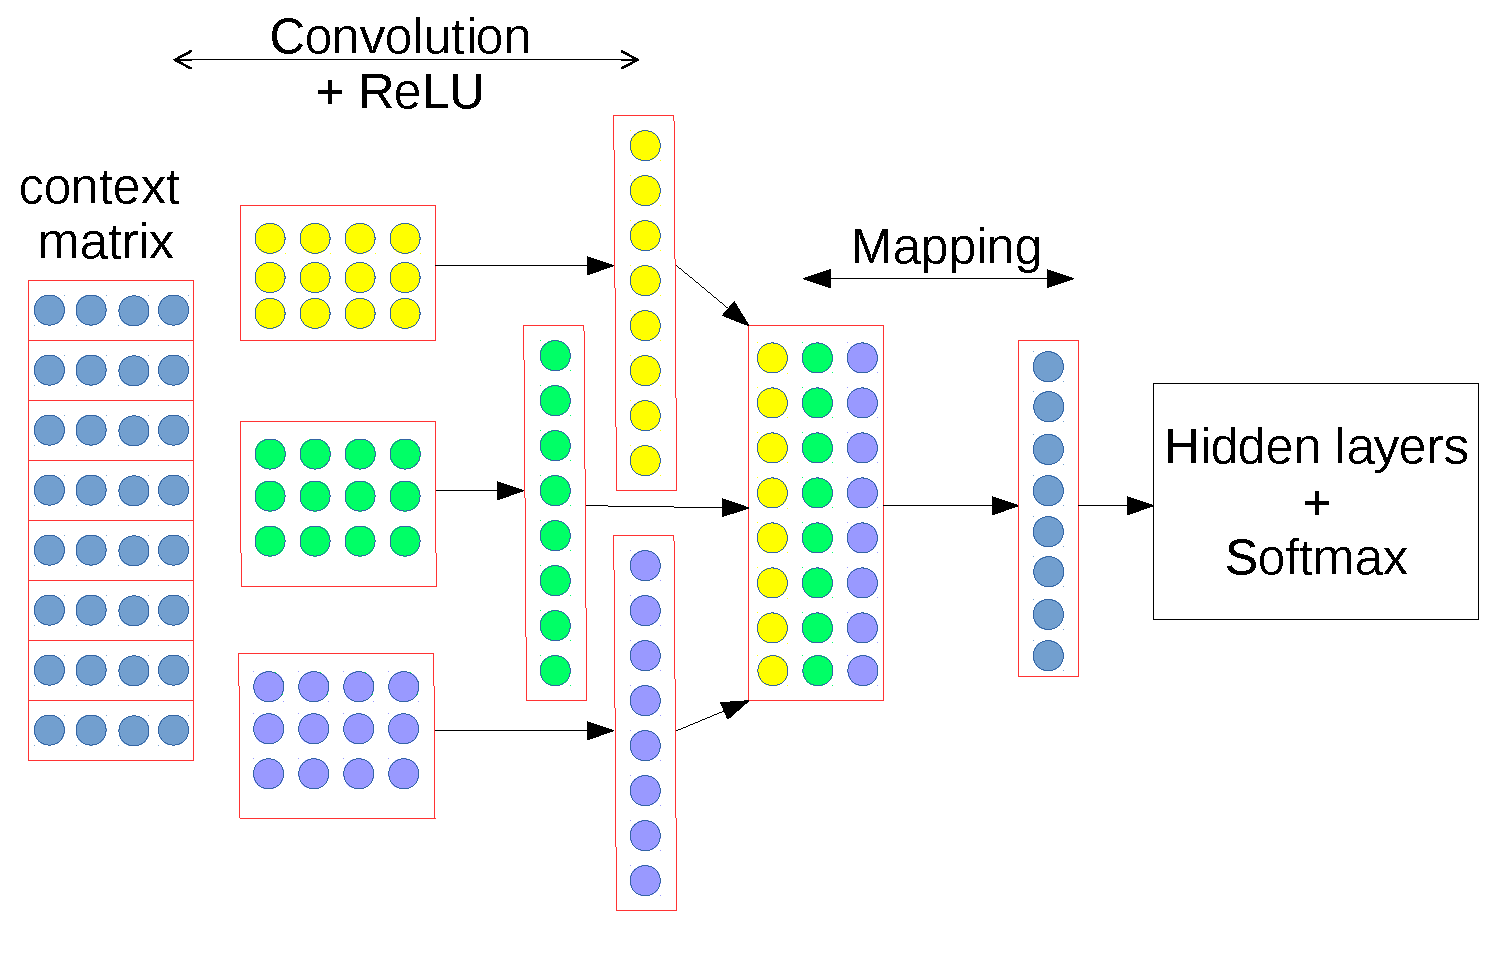
\includegraphics[width=\columnwidth]{figures/convolution.pdf}
~ \caption{Convolutional layer on top of the context matrix.}  
~ \label{fig:simpleconv}
~ \end{figure}
%
\begin{figure}[!t]
\centering
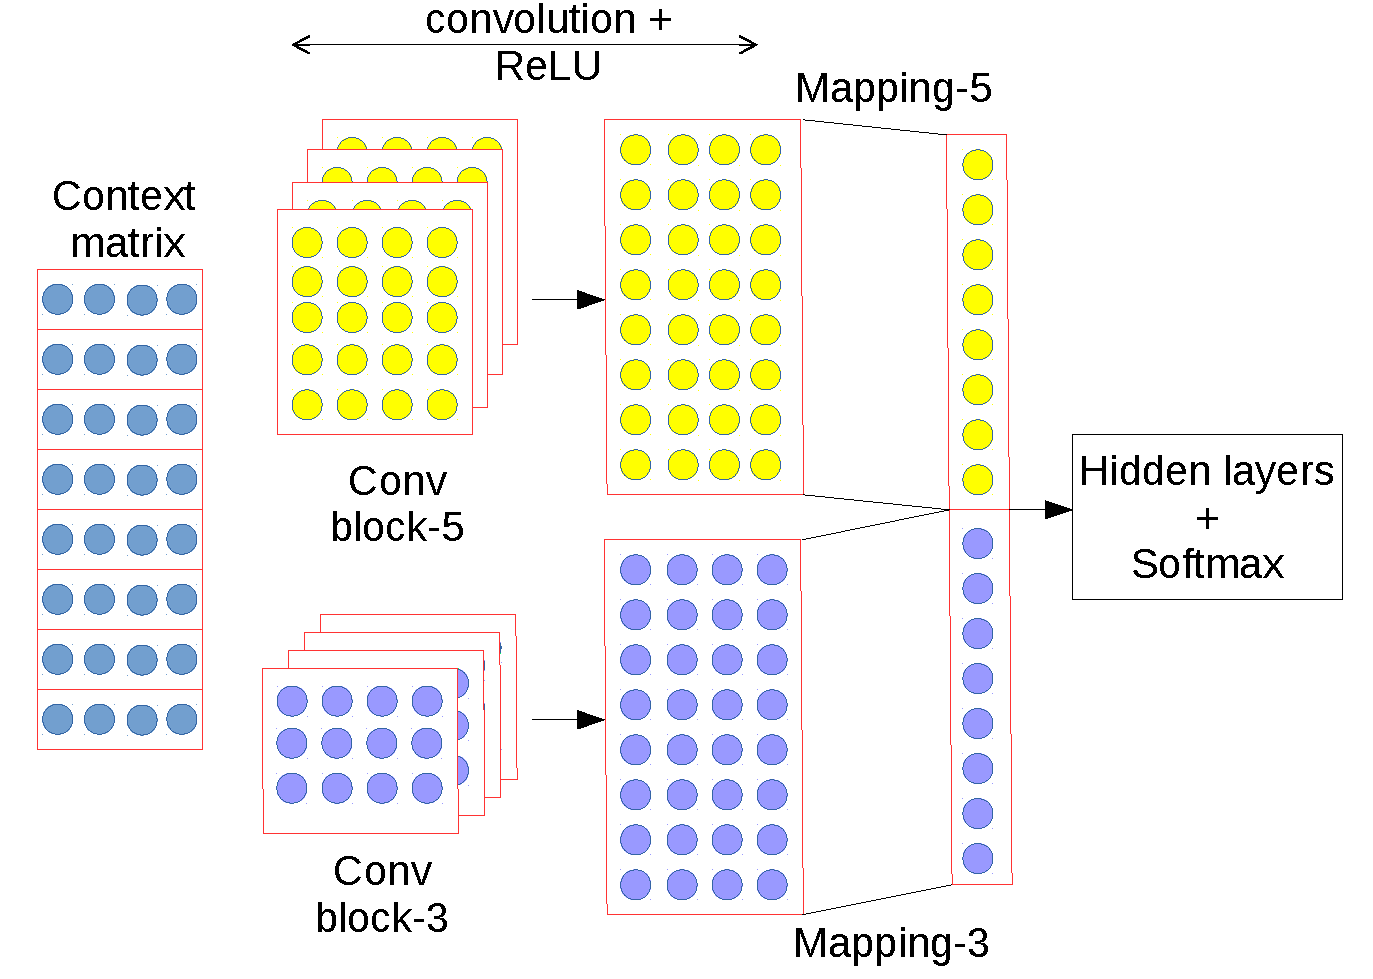
\includegraphics[width=\columnwidth]{figures/combine.pdf}
\caption{Combining kernels with different sizes. We concatenate the outputs of 2 convolutional blocks with kernel size of $5$ and $3$ respectively.}  
\label{fig:combine}
\end{figure}

\chapter{Experiments}
\label{c:exp}
We evaluate our model on two English corpora of different sizes and
genres that have been used for language modeling evaluation
before. The {\bf Penn Treebank} contains one million words of
newspaper text with 10K words in the vocabulary. We reuse the
preprocessing and train/test/valid division
from~\cite{mikolov2014learning}. 
%\gbt{Changed Europarl to Europarl-NC because Europarl usually refers
%to the multilingual Europarl corpus developed by I think Koehn ages
%ago.}
{\bf Europarl-NC} is a a 64-million word corpus that was developed for
a Machine Translation shared task~\cite{bojar-EtAl:2015:WMT},
combining Europarl data (from parliamentary debates in the European
Union) and News Commentary data.  We preprocessed the corpus with
tokenization and true-casing tools from the Moses
toolkit~\cite{koehn2007moses}. The vocabulary is composed of words
that occur at least 3 times in the training set and contains
approximately 60K words. %We use the validation and test set
% of the MT shared task.

We train our models using Stochastic Gradient Descent (SGD) and we
reduce the learning rate by a fixed proportion every time the
validation perplexity increases after one epoch. The values for learning rate,
learning rate shrinking 
%\gbt{isn't it ``learning rate decay''?}
and mini-batch sizes as well as context size are
fixed once and for all based on insights drawn from previous
work~\cite{le2011structured,sukhbaatar2015end,devlin2014fast} and
through experimentation with the Penn Treebank validation set. Experimentally we found SGD to be efficient and adequately fast, while other learning algorithms involve additional hyper parameters (such as alpha in RMSprop~\cite{tieleman2012lecture})

%For parameter tuning, we are concerned with trying the parameters which are less
%data-dependent including learning rate, learning rate shrink and mini-batch size on the small
%corpus (Penntreebank) and then recycle them on experiments with larger corpora. 
%The choice 
%of parameters also refers to previous works in feed-forward networks~\cite{le2011structured,sukhbaatar2015end,devlin2014fast}.
Specifically, the learning rate is set to $0.05$, with mini-batch size
of 128 (we do not take the average of loss over the batch, and the
training set is shuffled). We multiply the learning rate by $0.5$
every time we shrink it and clip the gradients if their norm is larger
than $12$. The network parameters are initialized randomly on a range
from $-0.01$ to $0.01$ and the context size is set to $16$. In
Section~\ref{sect:ana} we show that this large context window is fully
exploited. 
%The property of neural networks allow us to use such large context. We
%also aim at finding if the network can take into account the context words from afar. 

For the base FFNN and CNN we study embedding sizes (and thus, number of kernels) $k=128,256$. For $k=128$ we explore the simple CNN, incrementally adding NIN and COM variations (in that order) and, alternatively, using a ML-CNN. For $k=256$, we only explore the former three alternatives. For the kernel size, we set it to $w=3$ words for the simple CNN (out of options $3,5,7,9$), whereas for the COM variant we use $w=3$ and $5$. However, we observed the models to be generally robust to this parameter. Dropout rates are tuned specifically for each combination of model and dataset based on the validation perplexity. We also add small dropout ($0.05-0.15$) when we train the networks on the small corpus (Penn Treebank). 

% Data-dependent parameters are word embedding $k$ (the size of hidden layers is scaled by $k$),
%and dropout. For each corpus, we started with a low embedding size then increased it exponentially.
%The dropout value is tuned on the validation data. We report the test perplexity (lower is better) after getting the best
%dropout value for the embedding size. The size of the network is also restricted by our computational resource.

The experimental results for recurrent neural network language models,
such as Recurrent Neural Networks (RNN) and Long-Short Term Memory (LSTM), on the Penn Treebank are quoted from previous
work; for Europarl-NC, we train our own models (we also report the
performance of these in-house trained RNN and LSTM models on the Penn Treebank for
reference). Specifically, we train LSTMs with embedding size $k=256$
and number of layers $L=2$ as well as $k=512$ with $L=1,2$. We train
one RNN with $k=512$ and $L=2$. To train these models, we use the
published source code from~\cite{zaremba2014recurrent}. Our own models are also
implemented in Torch7\footnote{We'll link the source code here if the paper is accepted} %available at https://github.com/quanpn90/convlm.} 
	for easier comparison.

 For all models trained on Europarl-NC, we used hierarchical softmax to
speed up training, clustering the words in the vocabulary into 245
classes based on word frequency.

%~ \gbt{What vocabulary size?};
%~ {\bf Text8}, comprising the first 17 million words from a Wikipedia
%~ dump with about $44$K words in the vocabulary (also used
%~ in~\newcite{mikolov2014learning}); and a 64-million word corpus ({\bf
  %~ Europarl-NC}) combining \gbt{pls check} Europarl data (from
%~ parliamentary debates in the European Union) and News Commentary
%~ monolingual data \gbt{what kind of genre is that?} that was developed
%~ for a Machine Translation shared task~\cite{bojar-EtAl:2015:WMT}.

%~ For the first two corpora, we reuse the preprocessing steps
%~ in~\cite{mikolov2014learning}. For Europarl-NC, after preprocessing the
%~ corpus with tokenization and true-casing with tools provided in the
%~ Moses toolkit~\cite{koehn2007moses}, we selected the words that appear
%~ at least 3 times in the training set to obtain a vocabulary of
%~ approximately $60K$ words.

%~ To implement our models, we
%~ used Torch 7~\cite{collobert2011torch7} because of its fast CNN
%~ modules. We also used the implementation of LSTM/RNN language models
%~ in~\cite{zaremba2014recurrent} for the comparative experiments.

%~ As mentioned above, we fix the number of kernels in each convolutional
%~ layer to be equal to the embedding dimensionality $k$. Furthermore,
%~ the size of the first hidden layer --after the projection in the FFLM
%~ or after the convolutional layer in the CNN-- is also kept at
%~ $2 \times k$. We did not tune this parameter, but rather report
%~ results for different choices of $k$.

 %For example, \`baseline-128\' refers to the feed-forward model with embedding size of $128$ and hidden layer size of $256$. The upgraded CNN model has one more convolutional layer with $256$ feature maps. The second improvement comes from the Network-in-Network (``+Nin'') structure applied to the convolutional kernel. 
 %The kernel window size and padding parameters are adjusted so that the convolutional outputs have the same size as the embedding inputs, after simple reshaping.

%~ As mentioned above, we fix the number of kernels in each convolutional
%~ layer to be equal to the embedding dimensionality $k$. Furthermore,
%~ the size of the first hidden layer --after the projection in the FFLM
%~ or after the convolutional layer in the CNN-- is also kept at
%~ $2 \times k$. We did not tune this parameter, but rather report
%~ results for different choices of $k$.
%For example, \`baseline-128\' refers to the feed-forward model with embedding size of $128$ and hidden layer size of $256$. The upgraded CNN model has one more convolutional layer with $256$ feature maps. The second improvement comes from the Network-in-Network (``+Nin'') structure applied to the convolutional kernel. 
%The kernel window size and padding parameters are adjusted so that the convolutional outputs have the same size as the embedding inputs, after simple reshaping. 
%~ {\bf FIXME: In section 3.2 explain that the window is centered on the the input $i$ and padding vectors are added before and after the full context}
%~ Other parameters we explore are window size (${3, 5, 7}$), dropout
%~ probability values (from $0.1$ to $0.5$ \gbt{check} in steps of $0.1$), and the number of
%~ convolutional layers (${1. 2}$) \gbt{I don't understand
  %~ ${1. 2}$}. \gbt{check following} The weights of the network are
%~ randomly initialised from a uniform distribution of values between
%~ $-0.01$ and $0.01$ based on other works in
%~ FFLM~\cite{schwenk2007continuous}. For the convolutional weights, we
%~ found that the presence of Batch Normalisation reduces the effect of
%~ the initialisation method. We do not observe any difference between
%~ using the initialization just described (randomly drawn from a uniform
%~ distribution $-0.01 - 0.01$) and the MSR initialization
%~ method~\cite{he2015delving}.

%~ \gbt{Quan, has the move requested in the commented-out text below been done? but I think that the
%~ ReLU information does belong here}
% {\bf $<$begin move to Section 3$>$}  Notably, dropout is only applied to the fully connected components, thus having no effect on the convolutional layer. The activation function used in all experiments is ReLU. Not only can ReLU avoid gradient saturation, the activated neurons always have positive values, this facilitating the analysis of subsequent hidden layers. {\bf $<$/end move to Section 3$>$}

%~ Regarding the context size, we use $16$ words in the context for most
%~ of our experiments.  {\bf $<$begin move to Section 1 or 3$>$ (as
  %~ motivation for CNN)} Neural network language models, by their
%~ nature, can scale up the distribution for an arbitrary context size,
%~ which could be too sparse for count-based
%~ models~\cite{kneser1995improved}. It is notable, however, that the
%~ feed forward models in~\cite{hai2012measuring} do not benefit much
%~ from a context larger than $10$, yet the author only took into account
%~ the words in the current sentence \gbt{I don't understand from ``yet''
  %~ to here}.  {\bf $<$/end move to Section 1 or 3$>$} We empirically
%~ choose the size of each mini-batch (shuffled during training) as $128$
%~ {\bf how were the parameters calibrated?} and update the parameters
%~ with simple mini-batch gradient descent. The learning rate is
%~ initially set to $0.05$ and gradually decreased by $2$ \gbt{you mean
  %~ halved, right? -- ``decreased by $2$'' ambiguous} when the
%~ validation perplexity stops decreasing, following previous work for
%~ similar
%~ networks~\cite{le2011structured,sukhbaatar2015end,devlin2014fast} (we
%~ do not average the loss value over batches). Typically it takes
%~ approximately $30$ epochs for the models (including the baseline FFLM)
%~ to converge.

%~ The experimental results for Recurrent Neural Network language models
%~ are mostly quoted from previous works. We use the published source
%~ code from~\cite{zaremba2014recurrent} to produce the results
%~ for RNN and LSTM for the Europarl-NC corpus.

%~ As standard in language modeling, we report perplexity \gbt{brief
  %~ description, no need for formula.} (lower is better). 



\chapter{Model Analysis}
\label{c:analysis}

\begin{figure*}[!t]
\centering
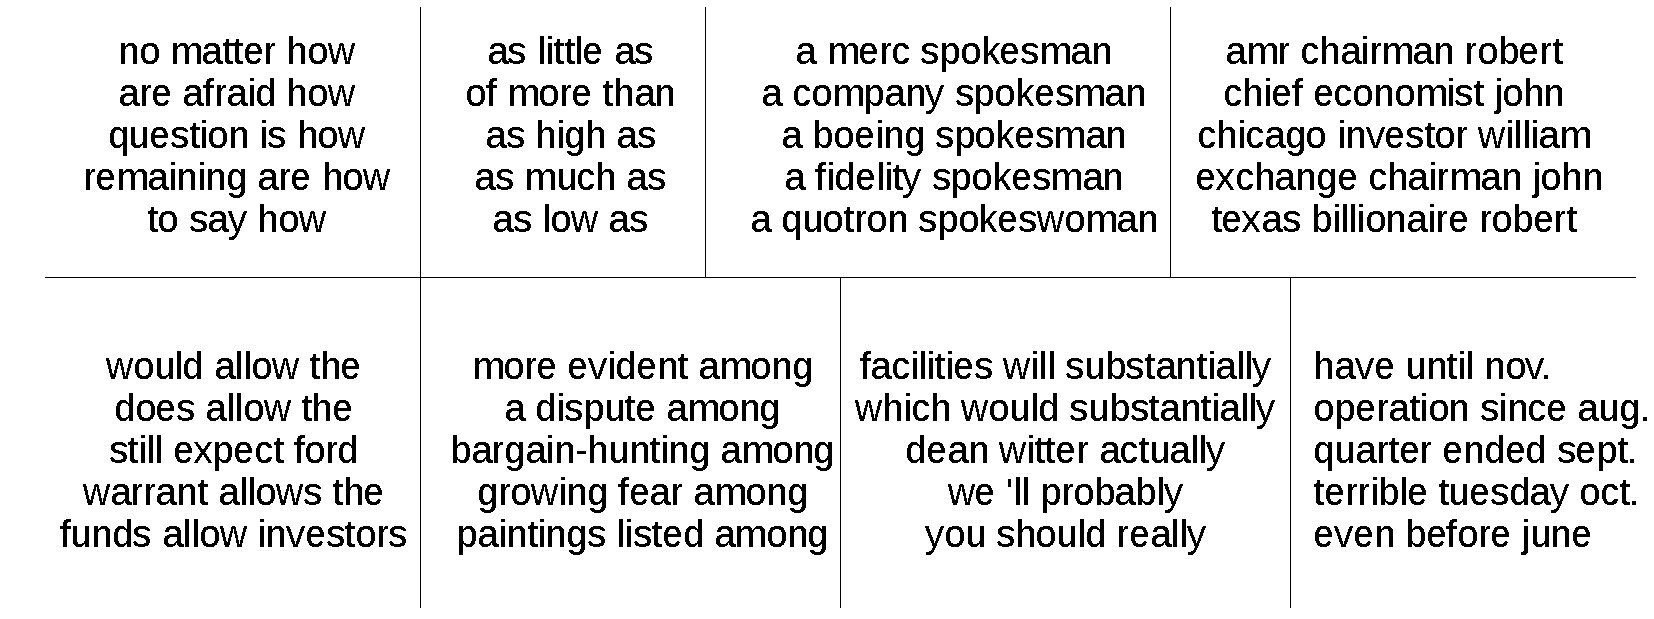
\includegraphics[width=\textwidth]{figures/kernels.pdf}
\centering
\caption{Some example phrases that have highest activations for 8 example kernels (each box), extracted from the validation set of the Penn Treebank. Model trained with 256 kernels for 256-dimension word vectors.}  
\label{fig:kernels}
\end{figure*}

In what follows, we obtain insights into the inner workings of the CNN by looking into
the linguistic patterns that the kernels learn to extract and also studying
the temporal information extracted by the network in relation to its prediction capacity.

\paragraph{Learned patterns} 
To get some insight into the kind of patterns that each kernel is
learning to detect, we fed trigrams from the validation set of the
Penn Treebank to each of the kernels, and extracted the ones that most
highly activated the kernel. Some examples are shown in
Figure~\ref{fig:kernels}. Since the word windows are made of
embeddings, we can expect patterns with similar embeddings to have
close activation outputs.
%~ \gbt{inventing wildly, check following} 
This is borne out in the analysis: The kernels specialize in distinct
features of the data, including more syntactic-semantic constructions
(cf.\ the ``comparative kernel'' including \emph{as \dots as}
patterns, but also \emph{of more than}) and more lexical or topical
features (cf.\ the ``ending-in-month-name'' kernel). Even in the more
lexicalized features, however, we see linguistic regularities at
different levels being condensed in a single kernel: For instance, the
``spokesman'' kernel detects phrases consisting of an indefinite
determiner, a company name (or the word \emph{company} itself) and the
word ``spokesman''. We hypothesize that the convolutional layer adds
an ``I identify one specific feature, but at a high level of
abstraction'' dimension to a feed-forward neural network, similarly to
what has been observed in image
classification~\cite{krizhevsky2012imagenet}.

%~ We assume that, the
%~ convolutional layers altered the values of word embeddings from
%~ \textbf{globally independent} to \textbf{regional values}. \gbt{I
  %~ don't understand this latter sentence. Pls expand.}

%~ \textbf{Kernel size effect} By increasing the size of convolutional
%~ kernels, we want the kernels to learn longer $n$-gram patterns which
%~ can account more complicated phrases. Empirically, we observe that $3$
%~ and $5$ are the optimal kernel size for all of our experiments in all
%~ corpora (results are almost similar). Enlarging the window leads to
%~ the linear increase in the number of convolutional parameters and
%~ complexity, while we did not experience any improvement in
%~ perplexity. Possibly changing the window size requires the
%~ corresponding change in stride and padding, because at stride $= 1$,
%~ two neighbor windows have too much similar content.

%~ \textbf{Multi-layer convolution} \gbt{Why is this in the analysis
  %~ section? It belongs to the experiments section, right?}  With that
%~ interpretation \gbt{What interpretation?}, each convolutional layer is
%~ able to re-estimate embeddings at regional levels \gbt{?}. Therefore,
%~ additional convolutional layers can be applied on top of each other in
%~ order to connect local features, which has shown to be useful in the
%~ context in sentence representation~\cite{Kalchbrenner2014conv}. For
%~ language modeling, however, the performance of the models actually
%~ decreases with the number of layers (see
%~ Table~\ref{tab:ptblayers}). One reason could be the fact that language
%~ modelling contexts are mostly incomplete sentences, with a different
%~ nature than the complete sentences used for sentence
%~ representation. Moreover, stacking convolution layers can make the
%~ whole convolution block become too specific, in that it tries to
%~ remember the exact context in the training data. This may help explain
%~ why increasing the convolutional depth is not suitable for this
%~ particular problem, although further research is needed to test this
%~ claim.



% \gbt{This table was repeated, commenting it out just in case.}
% \begin{table}[tb]
%   \centering
%   \begin{tabular}{|c|c|c|}
%     \hline
%     Model & V & T\\
%     \hline 
%     Baseline ($k=128$) & 114 & 109 \\
%     +CNN ($1$ layer) & 102 & \textbf{97}\\
%     +CNN ($2$ layers) & 113 & 108 \\
% 	+CNN ($4$ layers) & 130 & 124 \\
%     \hline
%   \end{tabular}
% \caption{Performance on the Penn Treebank with different layers.}
% \label{tab:ptblayers}
% \end{table}


\begin{figure}[t]
	\centering
	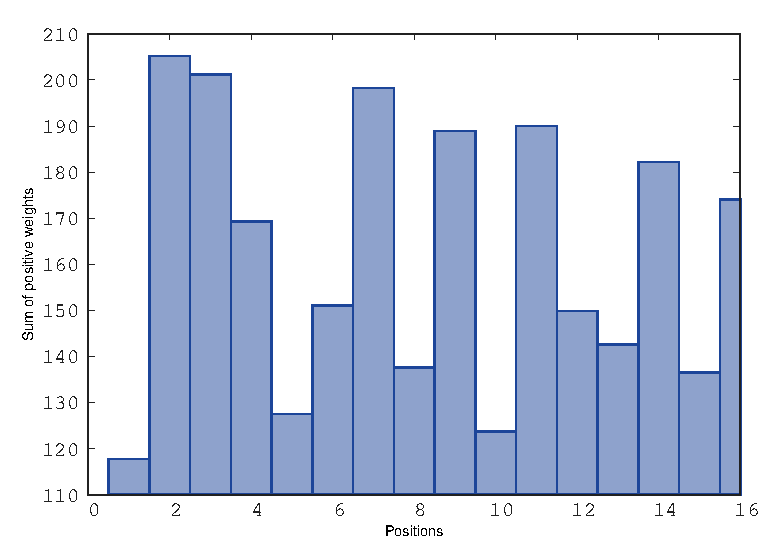
\includegraphics[width=\columnwidth]{figures/weight_dist.eps}
	\caption{The distribution of positive weights over context positions, where 1 is the position closest to the predicted word.}  
	\label{fig:weight-dist}
\end{figure}



\paragraph{Temporal information} To the best of our knowledge, the
longest context used in feed-forward language models is
$10$~\cite{hai2012measuring}, where no significant change in terms of
perplexity was observed for bigger context sizes, even though in that
work only same-sentence contexts were considered. In our experiments, we
use a larger context size of 16 while removing the sentence boundary limit
(as commonly done in $n$-gram language models) such that the network
can take into account the words in the previous sentences.

% We check whether our model \gbt{which version? And how
  %~ are the kernel values combined? E.g. what does the fact that the
  %~ number of active weights at position 3 is much smaller mean, is it
  %~ some effect of choosing kernel size 3? (but then what happens with
  %~ kernel 5?)} does profit from the information in the whole context
%~ through the following experiment:
To analyze whether all this information was effectively used,
 we took our best model, the CNN-NIN-COM model with
embedding size of 256 (fourth line, second block in
Table~\ref{tab:result}), and we identified the weights in the model
that map the convolutional output (of size $n \times k$) to a lower
dimensional vector (the ``mapping'' layer in
Figure~\ref{fig:simpleconv}). Recall that the output of the convolutional layer is
a matrix indexed by time step and kernel index representing the activation of
the kernel when convolved with a window of text centered around the given time step. Thus,
output units of the above mentioned mapping predicate over an ensemble of kernel activations for
each time-step . We can identify the
patterns that they learn to detect by extracting the time-kernel combinations
for which they have positive weights (since we have ReLU
activations, negative weights are equivalent to ignoring a
feature). 
First, we asked ourselves whether these units tend to be more
focused on the time-steps closer to the target or not. To test this,
we calculated the sum of the positive weights for each position in time using an average of the mappings that correspond to each output unit. %, even when the distribution of weights cannot allow us to obtain an attentional behaviour similar to the Memory Network~\cite{sukhbaatar2015end}.
The results are shown in
Figure~\ref{fig:weight-dist}. As could be expected, positions that are
close to the token to be predicted have many active units (local
context is very informative; see positions 2-4). However,
surprisingly, positions that are actually far from the target are also
quite active (see positions 10-14, with a spike at 11). It seems like the
CNN is putting quite a lot of effort on characterizing long-range
dependencies. %\newgk{This is not true, right?} Overall, the extent of activeness gradually reduces from the closest to the farthest position, which is in line with the previous work~\cite{hai2012measuring}. 
%Also, the effect of convolution is also reflected here, when the weights in the middle seem to fluctuate with the stride of the convolution. 

\begin{figure}[t]
	\centering
	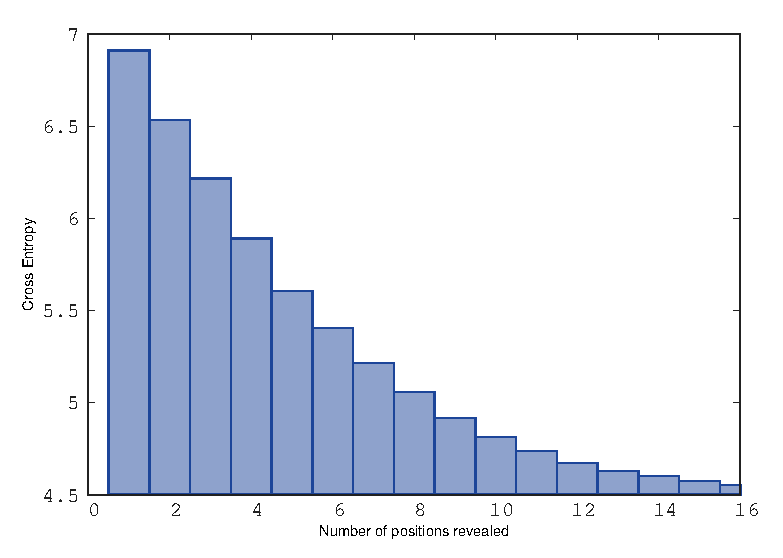
\includegraphics[width=\columnwidth]{figures/ppl_positions.eps}
	\caption{Perplexity change over position, by incrementally revealing the Mapping's weights corresponding to each position.}  
	\label{fig:position}
\end{figure}

Next, we checked that the information extracted from the positions
that are far in the past are actually used for prediction. To measure
this, we artificially lesioned the network so it would only read the
features from a given range of timesteps 
%\newgbt{check following}
(words in the context).  To lesion the network we manually masked the
weights of the mapping that focus on times outside of the target range
by setting them to zero. We started using only the word closest to the
final position and sequentially unmasked earlier positions until the
full context was used again. The result of this experiment is
presented in Figure~\ref{fig:position}, and it confirms our previous
observation that positions that are the farthest away contribute to
the predictions of the model. The perplexity drops dramatically as the
first positions are unmasked, and then decreases more slowly. However,
the last few positions still contribute to the final
perplexity. Indeed, the decrease almost follows a power-law
distribution, in which the perplexity decreases whenever we unmask a new position according to the following equation.

\begin{equation}
f(x) = 10e3 \times x^{-0.9}
\end{equation}



%~ \gk{Don't have the numbers here. Can you check if this is about right?}.


%\begin{itemize}
%\item First, we identified the weights in the hidden layer that map
%  the convolutional output from ($n \times k$)to a lower dimension
%  ($2 \times k$).
%\item Second, we masked the weights with zero, and then incrementally
%  unmasked the weights corresponding to each position, starting with
%  the one closest to the predicted word.
%\end{itemize}

%~ \gbt{Make font of axes in Figs 5, 6 larger (at least as large as
  %~ caption size). Also make ``plus'' signs larger. Why is there no
  %~ datapoint at position 16?}
%Figure~\ref{fig:position} records the perplexity change when unmasking
%the weights corresponding to each position. The perplexity drops
%dramatically in the first few positions, and then decreases more
%slowly; however, the last few positions still contribute to the final
%perplexity. 

%We also extracted the average number of positive weights on each position
%(Figure~\ref{fig:weight-dist}),indicating the
%number units that are active at each position. 
%  which showed that weights assigned for
% the last positions are quite active, while the most active area
% belongs to the closest positions to the predict words.
%~ \gbt{I'm inventing wildly in what follows, pls check.}  



%~ \textbf{Sampling}


\chapter{Related Works}
\label{c:related}

Convolutional Neural Networks (CNNs) were originally designed to deal
with hierarchical representation in Computer
Vision~\cite{lecun1995convolutional}. Deep convolutional networks have
been successfully applied in image classification and
understanding~\cite{karen2014vgg,kaiming2015resnet}. In such systems
the convolutional kernels learn to detect visual features at both
local and more abstract levels.
%A crucial difference between the aforementioned problems and language modeling is that 
%the context in each language modeling sample is normally not a full sentence. This property, together with temporal dependencies, makes 
%language modeling the more difficult task. 

%~ CNNs have also been applied directly on one-hot word vectors rather
%~ than word embeddings~\cite{johnson2015semi,johnson2015semi} in order
%~ to reduce the number of free parameters or over character
%~ embeddings~\cite{zhang2015text,yoon2015character}.
%In~\cite{zhang2015text}, the CNNs can operate on top of character sequences for classification. With the same approach,~\cite{yoon2015character} use time-delayed networks for word representation based on characters for better morphological discrimination. 

%The traits of our work are similar with Tag prediction from Twitter~\cite{weston2014tagspace}{\bf How?}. Besides, the memory network~\cite{sukhbaatar2015end} also shared some mechanical similarity with the convolutional networks, in which the context is scanned by the model multiple times for prediction{\bf Is this relevant?}. In~\cite{wang2015gen}, the author proposed a convolutional structure that can process contexts at any size, but the comparison between their model and the recurrent network is unclear, as well as their result is outperformed by our solid feed-forward baseline{\bf How does their model differ from ours?}.




In NLP, CNNs have been mainly applied to static classification task 
for discovering latent structures in text. \newcite{kim2014sentence} use a
CNN to tackle sentence classification, with competitive results. This
work also introduces kernels with varying window sizes to learn
complementary features at different aggregation
levels. \newcite{Kalchbrenner2014conv} propose a convolutional
architecture for sentence representation that vertically stacks
multiple convolution layers, each of which can learn independent
convolution kernels. CNNs with similar structures have also been
applied to other classification tasks, such as semantic
matching~\cite{hu2014convolutional},
%\gbt{what is semantic matching? we call it sentence matching in the intro}
relation extraction~\cite{nguyen2015relation} and information
retrieval~\cite{shen2014latent}.  In
contrast,~\newcite{collobert2011natural} explore a CNN architecture to
solve various sequential and non-sequential NLP tasks such as
part-of-speech tagging, named entity recognition and also language
modeling. This is perhaps the work that is closest to ours in the
existing literature. However, their model differs from ours in that it
uses a max-pooling layer that picks the most activated feature across
time, thus ignoring temporal information, whereas we explicitly avoid
doing so. More importantly, the language models trained in this work are only
evaluated through downstream tasks and through the quality of the
learned word embeddings, but not on the sequence prediction task
itself.

In this work we focus on statistical language modeling, which differs
from most of the tasks where CNNs have been applied before in multiple ways. First,
the input normally consists of incomplete sequences of words rather
than complete sentences. Second, as a classification problem, it
features an extremely large number of classes (the words in a large
vocabulary). Finally, temporal information, which can be safely
discarded in many settings with little impact in performance, is
critical here: An $n$-gram appearing close to the predicted word may
be more informative, or yield different information, than the same
$n$-gram appearing several tokens earlier.

\chapter{Conclusion}
\label{c:conc}
In this work, we have investigated the use of Convolutional Neural
Networks for language modeling, a sequential prediction task.
%\newgbt{for the future}
%To this end we extended earlier feed-forward language models with
%current techniques to obtain a base model that yields competitive
%results from the start.
We incorporate a CNN layer on top of a strong feed-forward model
enhanced with modern techniques like Highway Layers and Dropout. Our results
show a solid 13\% improvement in perplexity with respect to the
feed-forward model across two corpora of different sizes and genres 
when the model uses Network-in-Network 
and combine kernels of different window sizes. However, even without these additions
we show CNNs to effectively learn language patterns to significantly 
decrease the model perplexity.

In our view, this improvement responds to two key properties of CNNs,
highlighted in the analysis. First, as we have shown, they are able to
integrate information from larger context windows, using information
from words that are as far as 16 positions away from the predicted
word. Second, as we have qualitatively shown, the kernels learn to
detect specific patterns at a high level of abstraction. This is
analogous to the role of convolutions in Computer Vision. The analogy,
however, has limits; for instance, a deeper model stacking convolution
layers harms performance in language modeling, while it greatly helps
in Computer Vision. We conjecture that this is due to the differences
in the nature of visual vs.\ linguistic data. The convolution creates
sort of abstract images that still retain significant properties of
images. When applied to language, it detects important textual
features but distorts the input, such that it is not text anymore.
%described a variant of feed-forward language models, in which the convolutional neural networks are used to improve local representation on top of 
%word embeddings. Despite the fact that language modeling is a difficult sequential task, the presence of convolutional neural networks is still empirically useful compared to 
%the feed-forward baseline, by performing competitively with the state-of-the-art models. 

As for recurrent models, even if our model outperforms RNNs, it is
well below state-of-the-art LSTMs. Since CNNs are quite different in
nature, we believe that a fruitful line of future research could focus
on integrating the convolutional layer into a recurrent structure for
language modeling, as well as other sequential problems, perhaps
capturing the best of both worlds.

% More importantly, despite the fact that convolutional and feed forward
% neural network in general are not as well designed as recurrent
% network for language modeling, we still manage to find setups that
% allow them to well perform. Further investigation of convolutional
% neural network can be useful for text understanding.

%%% Local Variables:
%%% mode: latex
%%% TeX-master: t
%%% End:

%~ \chapter{
%~ \chapter{Background}
%~ \label{c:background}
%~ This chapter describes the basic knowledge of Statistical Language Modeling together with the prominent approaches. The research context is 
drawn in order to show the necessity of the neural network-based approaches. 
\section{Statistical Language Modeling Overview}

Quality measurement of language models is often carried out using two different ways. First, statistical language models can be evaluated by the capability to predict a new corpus. The perplexity (PPL) of a word sequence~\textbf{$w_1^L$} is computed as follows.
\begin{equation}
\label{eq:ppl}
PPL = \exp(\frac{\sum_{l=1}^L{-\ln P(w_i|h_i)}}{L}  )
\end{equation}
It is notable that the exponential term is the average of the negative log-likelihood of every word in the data, while $\log_2 \text{PPL}$ is the \textbf{Entropy} of the model. A low perplexity value corresponds to the fact that the language model is able to fits better the data, since the distribution of the model is closer to the unknown distribution of the test data. 

Second, the quality of language models can also be evaluated through their impacts on other applications such as Automatic Speech Recognition (ASR) or Statistical Machine Translation (SMT), by reducing the errors in the output of such systems. Specifically, in ASR, the metric used to evaluate the contribution of language models is Word Error Rate (WER) which is the distance between the decoder hypothesis and the reference. Similarly in SMT, the effect of language models can be reflected by the BLEU score~\cite{papineni2002bleu} or even human judgement. 

The main advantage of perplexity is that it is fast to perform and independent to other complex systems. The crediablilty of perplexity, however, depends on the validation/test data as well as the underlying vocabulary. It is also unusable for models that provide unnormalised distributions (sum of the distributions does not equal to $1$). More importantly, an improvement in terms of perplexity does not always result in the application improvement. For example, the improvement is required to be at least $10\%$ to be noteworthy for an ASR system~\cite{Rosenfeld:2000}


\section{N-gram Models}

%\subsection{About language modeling}
In general, language models aim at measuring the fluency of any text, showing how much it makes sense. Artificial systems that generate text, therefore, requires
the aid of language models in order to produce textual outputs that are comprehensible. 

From the statistical point of view, a word string is considered as a stochastic process, thus the language model is formulated as the probability estimation over all 
possible sequences of words. The sequence length can be arbitrary, while the words are taken from a limited vocabulary. For example, the likeliness of "the end of our world" is much higher than "tea end of our word", because the latter string is much less likely to be found in available English text. 

Since direction estimation for that probability distribution is intractable, the probability of a sentence $P(w_1^L)$ is factorised using the chain rule:
\begin{equation}
\label{eq:lm1}
P(w_1^L) = P(w_1 | \text{\textless s\textgreater}) \prod_{i=2}^L P(w_i | \text{\textless s\textgreater} w_1^{i-1})\\
		 = \prod_{i=l}^L P(w_l | h_l)
\end{equation}
in which, \text{\textless s\textgreater} is used to denote beginning token of the sentence/string. The history $h_i$ represents the string before the current word $w_i$. Instead of directly modeling the original distribution, the statistical models estimate the constituent probabilities, which usually results in browsing or storing the statistics of millions of
possible word strings since each language may consist of several thousands to millions of words. 

%~ Application of language models
The language modeling problem has experienced many approaches over the last two decades, most of which aiming at maximising the log-likelihood of the data (minimising the perplexity at the same time), while using some constraints and techniques to generalise to unseen data. The most widely used models rely on $n$-grams based on the Markov assumption that each word depends on $n-1$ previous words. 

\begin{equation}
\label{eq:markov}
P(w_i|h_i) \approx P(w_i|w_{i-n+1}^{i-1})
\end{equation}

Count-based models estimate the probability of each $n$-gram based on simple counting. The method is unreliable since it struggles at estimating the distribution for rare and unseen $n$-grams, many of which actually make sense in natural language. Many techniques have been proposed to overcome this weakness, including the smoothing techniques (Witten-Bell, Good-Turing or Knesey-Ney) with back-off and interpolation (estimation based on lower order $n$-grams)~\cite{kneser1995improved,chen1999empirical,heafield2011kenlm,federico2008irstlm,ney1994structuring,witten1991zero}. However, even with complicated smoothing techniques, the main weaknesses of $n$-gram language models are still exposed.

% 2. Weakness 
First, each word in the vocabulary is treated as a totally discrete random variable without any linguistic feature associated. The model relies on statistical occurrences and ignores morphological, syntactic and semantic relationship, by which the lexicon is formulated. There are several attempts to incorporate the word similarity in $n$-gram based language models. Notably, the class-based language models~\cite{brown1992class,niesler1996variable} introduced word clustering and assumed that the distribution of unseen or rate words can be achieved by using the richer statistics from the corresponding class, which is less sparse than the word itself. Also, the structured language models~\cite{chelba2000structured,filimonov2009joint} tries to filter out irrelevant context words and focuses on important counterparts by using parse trees, which compensates the lack of syntactic information in $n$-gram models. Despite such efforts, the language modeling results were still unreliable compared to the Knesey-Ney smoothing technique. However, those works in the literature also suggests that the syntactic and semantic properties of words need to be automatically learned from the data. 
%
Second, $n$-gram language models struggle to model a long range dependency between the predicted word and the context. Due to the fact that each word in the vocabulary is a separated random variable, the number of parameters to be estimated (statistics of $n$-grams) grow exponentially with the size of context. The~\textit{the curse of dimensionality} refers to the fact that one needs more amount of training data in order to reliably estimate the model when the number of learned parameters increases. For example, if the vocabulary size is $10000$, the total number of $n$-grams for $n=6$ is $10^16$ theoretically, which is also the number of parameters to be estimated accordingly. Also, the Zipf's law~\cite{kingsley1932selective} indicates that only a small subset of the vocabulary accounts for most occurrences in the training data, thus it is almost impossible to have a training data that covers all possible $n$-grams. 

The neural network language model, as a consequence, is investigated in order to tackle both problems that traditional count-based models cannot solve. 




%~ The main disadvantage of this evaluation method is that full ASR or SMT systems are required for comparison, while perplexity can be quickly produced. Therefore, in the scope of the thesis, we use perplexity as the main evaluation metrics. 


%\section{Count-based approaches in Language Modeling}
%
%\subsection{$N$-gram statistical language models}
%The statistical methods are revised from equation~\ref{eq:lm1}, in which the probability of a sentence is factored into constituent conditioned probabilities. There are many approaches proposed to estimate those probabilities, however most of them revolve around \textbf{maximum likelihood} (MLE) of the training data together with \textbf{smoothing techniques} that help the models generalise better on unseen data. Such estimation is often done by collecting the word co-occurrence frequencies, with the important Markovian assumption that the history $h_i$ is limited to only $n - 1$ words (thus called $n$-gram models):
%\begin{equation}
%\label{eq:markov}
%P(w_i|h_i) \approx P(w_i|w_{i-n+1}^{i-1})
%\end{equation}
%In order to estimate each conditional probability by MLE, we simply count the number of occurrences of the $n$-grams and the history:
%\begin{equation}
%\label{eq:ngramMLE}
% P_{MLE}(w_i|w_{i-n+1}^{i-1}) = \frac {C(w_1^n)} {C(w_1^{n-1})}
%\end{equation}
%where $C(X)$ is the number of times that the string $X$ appears in the training data.
%
%A problem arises when we need to estimate the probability distribution of rare word strings or even $n$-grams that do not occur in the corpus. According to Zipf law~\cite{kingsley1932selective}, the frequency distribution of a word is reversely proportional to its rank in the frequency table. The $n$-gram models, consequently, underestimate or even give
%null probabilities for unseen $n$-grams which actually make sense in natural language. As a result, smoothing techniques, which aim at assigning probabilities for unseen entries, are employed in order to alleviate estimation of rare $n$-grams. In the following section, we describe the most successful method which has been considered the standard in $n$-gram language models: the interpolated Knesey-Ney smoothing technique~\cite{kneser1995improved}. 
%
%%~ \subsection{Back-off techniques}
%
%\subsection{Popular smoothing techniques}
%
%There are a number of smoothing techniques proposed for language modeling, most of which are described in the overview provided by Chen and Goodman, 1998~\cite{}
%
%\subsubsection{Absolute discounting}
%
%\subsubsection{Kneser-Ney smoothing}

%
%\subsection{Structured language models}
%Originally, statistical language models were not warmly welcomed by the linguistic community, as can be seen from the 
%statement of Chomsky: the notion of probability of a sentence is completely useless one. Essentially, $n$-gram models, which will be described in subsequent sections, 
%and their finite state machine variations are not able to represent linguistic patterns and long term dependency between words in a sentence, or in a broad context. 
%
%Structured language models involve using~\textbf{Context free grammars} to generate a syntax tree for the word string, in which the leaves represent the words and the 
%other nodes are non-terminal symbols. The generation process is statistically learned from a training corpus, so that the final score of the sentence is decided from the probabilistic
%derivations of the grammar. 
%
%Despite the fact that structured language models are much more linguistically related than the statistical counterpart, they were not able to prove their practicality. The approach itself seems to be questionable when applied to speech content where the speakers do not strictly follow grammatical rules. Moreover, grammar construction often requires the participation of expert linguists and native speakers of the language, thus the method is expensive when applied to other languages. 

%
%
%\subsection{Class based language models}
%
%\subsection{Maximum Entropy Language models}

\section{Neural Network Models}

\subsection{Feed-forward neural network models}
In this section, we describe the neural language models~\cite{bengio2006neural} (also known as continuous space language models), which are designed to fight the curse of dimensionality in the conventional approaches, by utilising two properties as follows
%In order to fight the curse of dimensionality described above, neural language models are designed to utilise two properties as follow:

\begin{itemize}
	\item Words are no longer discrete variables without any relationship to each other. Alternatively, they are represented as vectors in a continuous space, where similar words are neighbors, such approach is referred as~\textit{Distributed word representation} or~\textit{Word embedding}~\cite{bengio2003neural}. With such representation, each $n$-gram representation is a combination of the word vectors, which no longer grows exponentially when $n$ is increased and we can mathematically quantify word similarity. More importantly, the distributed representation has to be learned during the language model learning process. 
	
	\item With the words mapped into continuous vectors and the $n$-gram context is the combination of the word vectors, the estimation of the probability distribution of each $n$-gram becomes learning a smoothing function over the context vector and produces the probability for all possible words in the vocabulary. Both the word space and the smoothing function are represented in neural networks, in which they are learnable parameters. 
\end{itemize}

With such design, a neural language model, if successfully trained, can capture the linguistic regularities and generalise from the samples in the training data to similar $n$-grams. Ideally, the embeddings of similar words would have small distance between each other. Consequently, if we replace a word within an $n$-gram with a similar word, there is only a small change in the input of the network, which in turn does not make a great difference in the probability distribution at the output. For example, if the model has seen the phrase ``The cat is running'', it should be able to predict the probability of the phrase ``A dog is running'' even if the latter does not appear in the training data.

In the literature, distributional semantic models that approximate word meaning from the contextual information has been investigated for a long time~\cite{miller1991contextual}. Traditionally most models achieve word embeddings by collecting the occurrence statistics of context words and rely on re-weighting techniques for context informativeness. Distributed representation for generic discrete variables had also been used in neural network models~\cite{paccanaro2001learning}, while attempts to solve language modeling with neural network were also observed~\cite{schmidhuber1996sequential}. However, the standard feed-forward neural language models described in~\cite{bengio2003neural} was the first attempt to combine word embeddings that are automatically learned in neural network language models. 

\subsection{Standard architecture}

This section is dedicate to describe the very first neural language model, which is illustrated in Figure~\ref{fig:neuralBengio}. The model takes the context words as inputs and outputs the probability distribution for~\textit{all} words in the vocabulary. It consists of three basic components: the input layer, the hidden layer and the output layer. . The hidden layer can be extended to two or more layers which does not change the fundamental architecture. 

~ \begin{figure}[!t]
~ \centering
~ 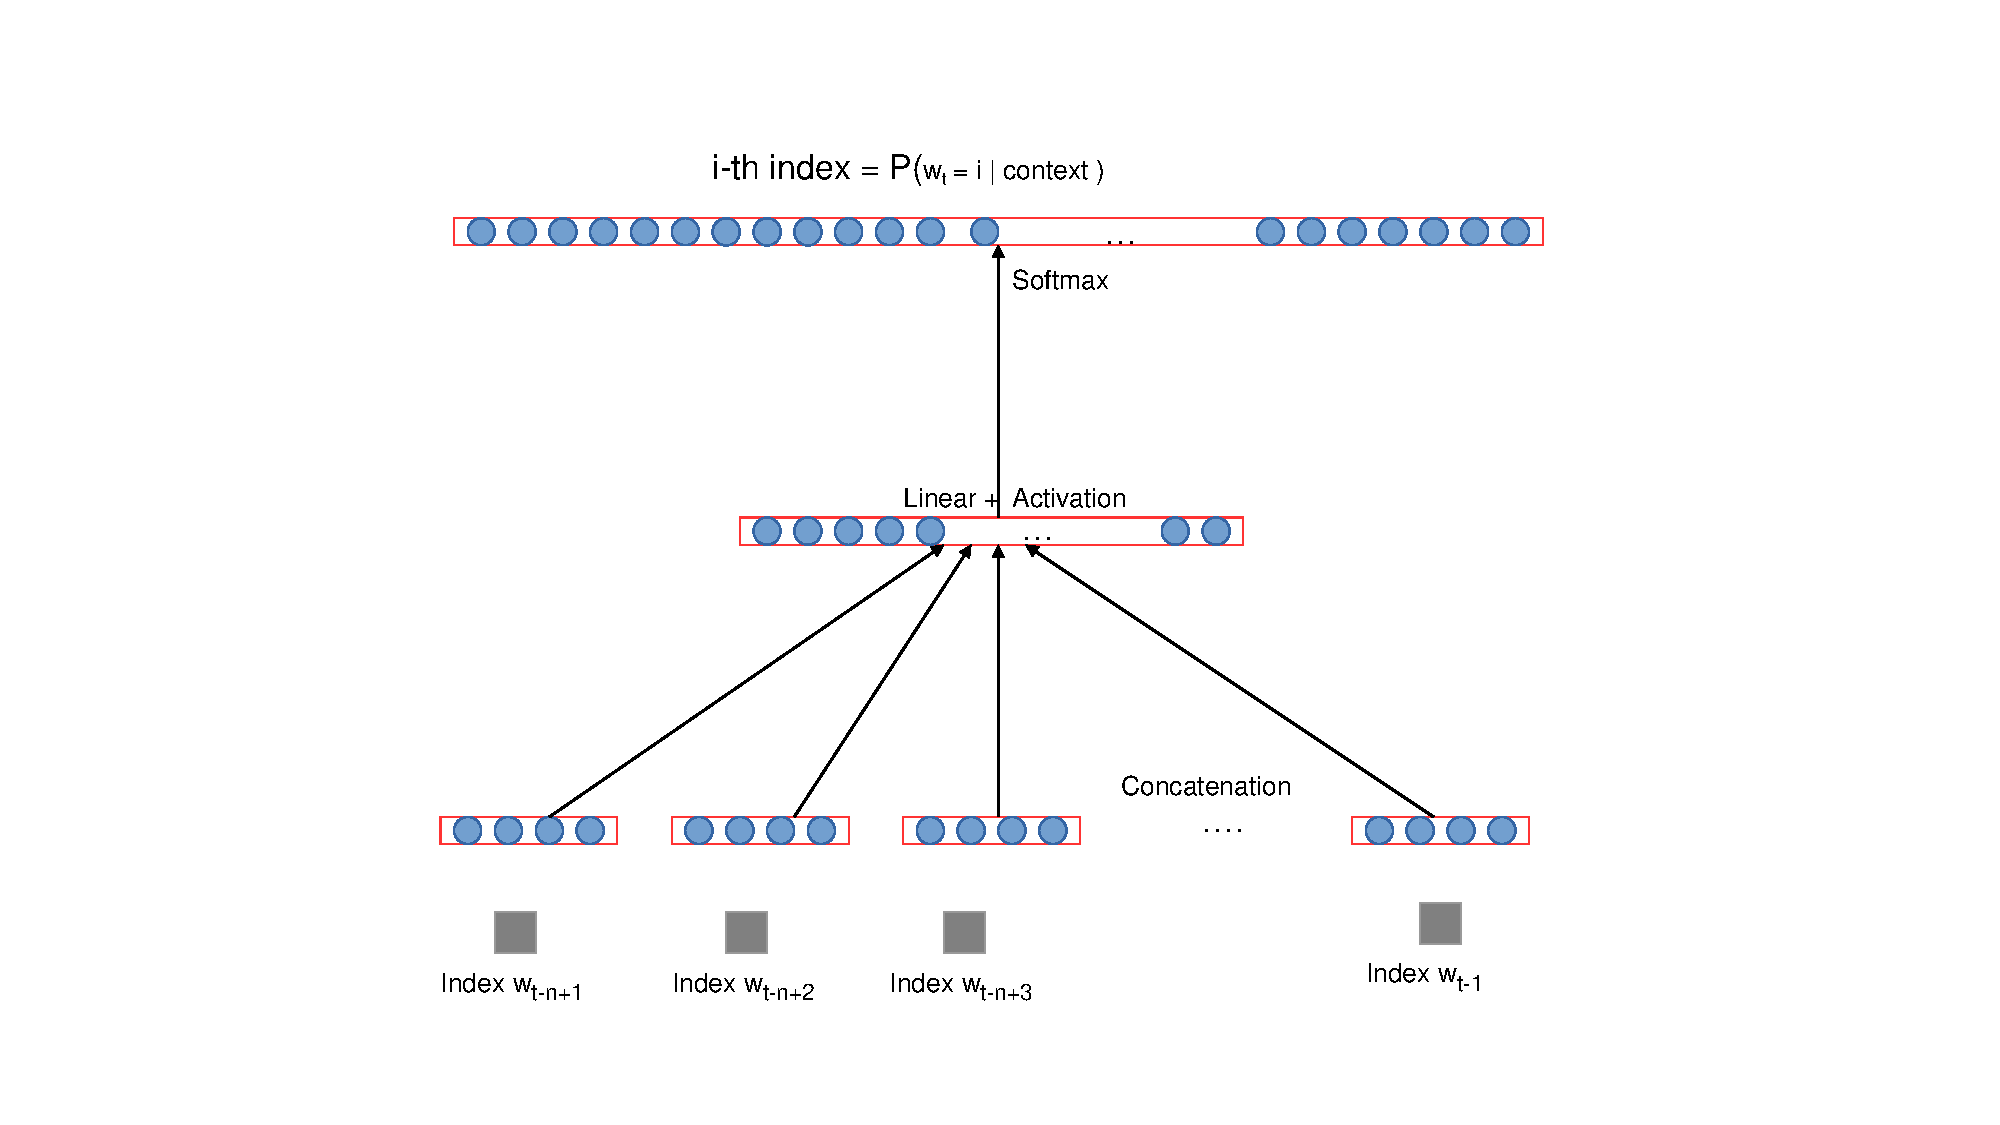
\includegraphics[width=\columnwidth]{figures/neuralLM.pdf}
~ \caption{Neural Language Model by Bengio et al~\cite{bengio2003neural}.}  
~ \label{fig:neuralBengio}
~ \end{figure}

\paragraph{Input layer}
The input layer constructs the embeddings of the words in the context, by using a shared word space and mapping each word in the context to a real-valued vector. Concretely, each word $w_i$ is represented as an 1-of-V coding, which is a long vector with the size of vocabulary V with all zeros except for the element corresponding to the word's index in the dictionary. Using this form of sparse coding, the word space (also called projection matrix $R$) is a matrix that contains V rows and each word embedding $v_i$ corresponds to one row of the matrix. The number of columns of the matrix is the size of the embedding, which is a tunable hyper-parameter. Notably, the values of the word vectors do not depend on the position of the word in the context. The context vector $i$ is the concatenation of the word vectors.

\begin{equation}
\begin{aligned}
i = \{R^T v_1; R^T v_2; .... ; R^T v_{n-1} \}
\end{aligned}  
\end{equation}


\paragraph{Hidden layer}
In the hidden layer, the input (context vector) is transformed nonlinearly, where each layer activation values are defined by

\begin{equation}
\begin{aligned}
h^j_{out} = f(W^j h_{in} + b^j) \\
h^1_{in} = i
\label{eq:hidden1}
\end{aligned}  
\end{equation}

In equation~\ref{eq:hidden1}, each hidden layer $h^j$ has the corresponding weights $W^j$ and $b^j$. The input of the first hidden layer is the context vector produced from the input (projection) layer. The size of the subsequent hidden layers are tunable hyper parameters. $f$ denotes a nonlinear activation function. Popular choices for the activation function are Tangent Hyperbolic, Sigmoid or ReLU, expressed in equation~\ref{eq:activation}. 


\begin{equation}
\begin{aligned}
 f(x) = 
	\begin{cases}
	\frac{\exp (x) - \exp (-x)}{\exp (x) + \exp (-x)}    \text{    if } f = \text{Tanh} \\
	\frac{1}{1 + \exp(-x)}                \text{     if } f = \text{Sigmoid} \\
	\max(0, x) \text{     if } f = \text{ReLU} \\
	\end{cases}
\label{eq:activation}
\end{aligned}
\end{equation}

\paragraph{Output layer}
The final layer of the network produces the probability distribution for all words in the vocabulary, thus having totally V nodes. Each neuron in the layer is associated to the probability of one word, as shown in Figure~\ref{fig:neuralBengio}. First, a linear transformation is used to obtain the unnormalised distribution:

\begin{equation}
\begin{aligned}
o = W^o h + b^o
\label{eq:linearoutput}
\end{aligned}  
\end{equation}

Notably, the values of $o$ is unnormalised because each element in o is associate to the score of each output word given the context vector. $W^o$ and $b^o$ are the corresponding weights and biases of the layer. Importantly, $W^o$ has the same form as the projection matrix at the input layer, since it also learns embedding for each word in the output vocabulary. Subsequently, the true probability distribution is estimated thanks to the~\textit{softmax} function:

\begin{equation}
p(w_i | h) = \frac{\exp(o_i)}{\sum_j \exp(o_j)}
\label{eq:softmax}
\end{equation}

In equation~\ref{eq:softmax}, the probability of each word $w_i$ given the encoded context $h$ is estimated by normalizing all values in $o$. Overall, the main tunable hyper-parameters of the network are the order of $n$-grams (the number of words in the context, which can range from 6 to 15), the sizes of hidden layers, and the word embedding size. The free parameters~$\Theta$ that are algorithmically learned from the data includes the projection matrix $R$, the weight matrices $W^h$ at the hidden layers, $W^o$ at the output layer and the biases $b^h$, $b^o$. 


\subsection{Training method}
From the machine learning perspective, the neural network language model has transformed the statistcal language modeling problem from a generative learning process to a discriminative classification problem. The free parameters of the network are trained by minimising the objective function, which is the log-likelihood~$\mathcal{L}$ of the  parameters~$\Theta$ given the training samples. The parameters are updated after each iteration based on some optimization techniques, among which Stochastic Gradient Descent (SGD) is most commonly used in neural language models \cite{zaremba2014recurrent,le2011structured,mikolov2010recurrent}. SGD and other variants such as Adadelta~\cite{zeiler2012adadelta} or RMSProp~\cite{tieleman2012lecture} require the computation of the first order derivatives of the loss function with respected to the parameters, which can be performed efficiently with the back-propagation algorithm~\cite{le1990handwritten}.

\subsection{Optimisation Process}
In this section, we describe the back-propagation flow in the standard feed forward neural language model - the core of the optimisation process. Back-propagation~\cite{rumelhart1985learning} involves using a dynamic programming strategy to compute the derivatives of the loss function with respect to the parameters layer by layer, based on the chain rules. In the standard network, the error derivatives are back-propagated from the output layer to the input (projection) layer.

\paragraph{Objective Function}

The smoothing function that we approximate with the neural network has parameters that can be iteratively tuned in order to~\textbf{maximise the log-likelihood of the training data}. 

The network aims at maximising the probability of the label word given the context, hence the objective function is typically chosen as the Negative Log-Likelihood function. Assuming we have N samples, each of which is an $n$-gram, we can compute the loss function over the training data as follows:

\begin{equation}
\mathcal{L} = - 	\sum_{i}^N \ln P( w_i | w_{i-n+1}^{i-1} ) \\
\label{eq:objective}
\end{equation}

The objective function is in line with the perplexity that we want to minimise (which is equivalent with maximising the log-likelihood of the training data). For ease of understanding, we denote the derivative of the loss function~$\mathcal{L}$ at~\textit{each} sample or batch of samples with respect to a variable $x \in \Theta$ by $dx$.  

For each sample, let's $w$ be the index of the predicted word $w_i$ in the vocabulary, we have:

\begin{equation}
\begin{aligned}
- \log P(w_i |  w_{i-n+1}^{i-1})  = - \log P(w | h) \\
= - log (\frac{\exp (o_w)}{\sum_i exp(o_i)}) \\
=  log(\sum_i \exp(o_i)) - o_w
\label{eq:objective2}
\end{aligned}
\end{equation}

Subsequently, we compute the error derivatives $dx$ given the parameters in each layer using back-propagation:

\paragraph{Output layer}

The derivatives at the output layer:

\begin{equation}
do_i = 
\begin{cases}
1 - p_i \text{ if } i == w \\
-p_i \text{     otherwise}
\end{cases}
\end{equation}

Notably, $o_i$ denotes the $i^{th}$ element of the vector $o$, which is the unnormalised distribution of the vocabulary given the encoded context $h$. 

\paragraph{Hidden layers}
As a result, we can compute the derivatives with respect to the parameters and the previous hidden layer $h$, based on the original inference from Equation~\ref{eq:linearoutput}. 

\begin{equation}
\begin{aligned}
dW^o = doh^T \\
db^o = do \\ 
dh = {W^o}^Tdo \\
\end{aligned}
\end{equation}


For the inner hidden layers, the  derivatives for the linear components are computed similarly, by replacing $do$ with $dh$ (the output of the previous hidden layer is the input of the next hidden layer). However, we have to take into account the non-linear activation functions, which are shown in the inference equation for the previous hidden layers:

\begin{equation}
h_{next} = f(W^h h_{prev} + b^h)
\end{equation}

With $W^h$ and $b^h$ are the corresponding weights connecting $h_prev$ to $h_next$. The derivatives are computed as follows:

\begin{equation}
\begin{aligned}
d[W^h h_{prev} + b^h] = f'(h_{next}) dh_{next} \\
db^h = d[W^h h_{prev} + b^h] \\
dW^h = d[W^h h_{prev} + b^h]h_{prev}^T \\
dh_{prev} = {W^h}^T d[W^h h_{prev} + b^h]
\label{eq:dhidden}
\end{aligned} 
\end{equation}

The derivative function of $f$, $f'$:

\begin{equation}
\begin{aligned}
f(x) = 
\begin{cases}
1 - \text{Tanh}(x)^2   \text{    if } f = \text{Tanh} \\
\text{Sigmoid}(x) - \text{Sigmoid}(x)^2                \text{     if } f = \text{Sigmoid} \\
1 \text{ when } x > 0 \text{ and 0 otherwise}  \text{     if } f = \text{ReLU} \\
\end{cases}
\label{eq:dactivation}
\end{aligned}
\end{equation}


\paragraph{Input Layer}

The derivative function of the input layer is identical to Equation~\ref{eq:dhidden} and Equation~\ref{eq:dactivation}, considering that the input layer is the layer before the first hidden layer. 

\paragraph{Parameter Update}

After obtaining the derivatives of the loss function with respect to all parameters in the network, we can update the parameters following Stochastic Gradient Descent. The method is based on the phenomenon that the gradient of a function always points towards the direction of maximal increase at any point. The update rule is as follows with the learning rate parameter $\alpha > 0$:

\begin{equation}
x = x - \alpha dx
\label{eq:sgd}
\end{equation}

The learning rate is also considered as a function of the number of samples trained in the data. Typically, the learning rate is updated after the model observes a number of training examples, with two most common ways. The first way is to exponentially decrease the learning rate after some training samples with a~\textit{learning rate decay}, normally an epoch (training all samples in the training data). The second way is to reduce the learning rate based on a validation data. After each epoch, if the perplexity on the validation data is decreased, the learning rate is kept the same, otherwise it is multiplied by the learning rate decay.


\subsection{Recurrent Neural Language Models}

Compared to the statistical $n$-gram models, the feed-forward neural language models had created a considerable leap in representation by combining distributed representation of words with a robust classifier to generalise from observed sequences. As can be seen from various works~\cite{schwenk2007continuous,le2011structured}, the feed-forward language model significantly outperformed the traditional Knesey-Ney back-off models. However, the feed-forward models require a fixed input size, thus still rely on the Markov Assumption which limits the context to a particular number of words, even when the context size can be huge up to $10$. In order to model long sentences, or even paragraphs with long-term dependencies, it is beneficial to investigate in models that can be flexible in terms of input size. For example, if the distance between the open bracket and the closed counterpart is further than the $n$-gram input size, the feed forward model may forget to close the brackets after seeing the initial one. Ideally, as the learning process of human is associated with a memory that keeps the current information (such as topics), similar structure should be simulated and integrated in the network.

\paragraph{Recurrent Neural Networks} RNN~\cite{elman1990finding} are a class of neural networks that can efficiently model sequences by using a dynamic memory structure. While the feed-forward network can only receive one input and compute the corresponding output without any relation with other inputs, the recurrent counterpart takes the input as a~\textit{series of time step}  $x_1, x_2, \dots, x_n$ and processes them one by one, taking into account the information stored in the previous steps. Concretely, for each input $x_i$, the network updates the hidden memory $h_i$ based on the previous one $h_{i-1}$. 

%The ''Vanilla`` model~\cite{elman1990finding} uses a simple combination of the input and the previous memory:

\begin{equation}
h_i = \mathcal{F}(x_i, h{i-1})
\end{equation}

 We will cover some popular RNN variations in the upcoming sections. In general, the strong point of these models lie in the ability to dynamically model sequences with arbitrary length, which the feed-forward neural networks cannot achieve. The advantage comes with the cost that the recurrent models are generally hard to train, due to the properties of back-propagation. A change in an arbitrary position of the sequence can lead to a change in the objective function, therefore training methods for RNNs typically have to trace back the previous time steps. In other words, the RNNs are equivalent to feed-forward neural networks with many hidden layers that share parameters across each other. Importantly, the model capacity of RNNs do not depend on the length of the sequences, but in the recurrence mechanism - the way the hidden layers are updated. 
 
\paragraph{Recurrent Language Models} Language Modeling can be viewed as a sequence modeling problem, in which each time step corresponds to one word. The first recurrent language model (RNNLM)~\cite{mikolov2010recurrent} employed the ``Vanilla'' model of Elman et al~\cite{elman1990finding} as can be seen in Figure~\ref{fig:SimpleRNN}, in which the hidden steps are updated as follows:

~ \begin{figure}[!t]
	~ \centering
	~ 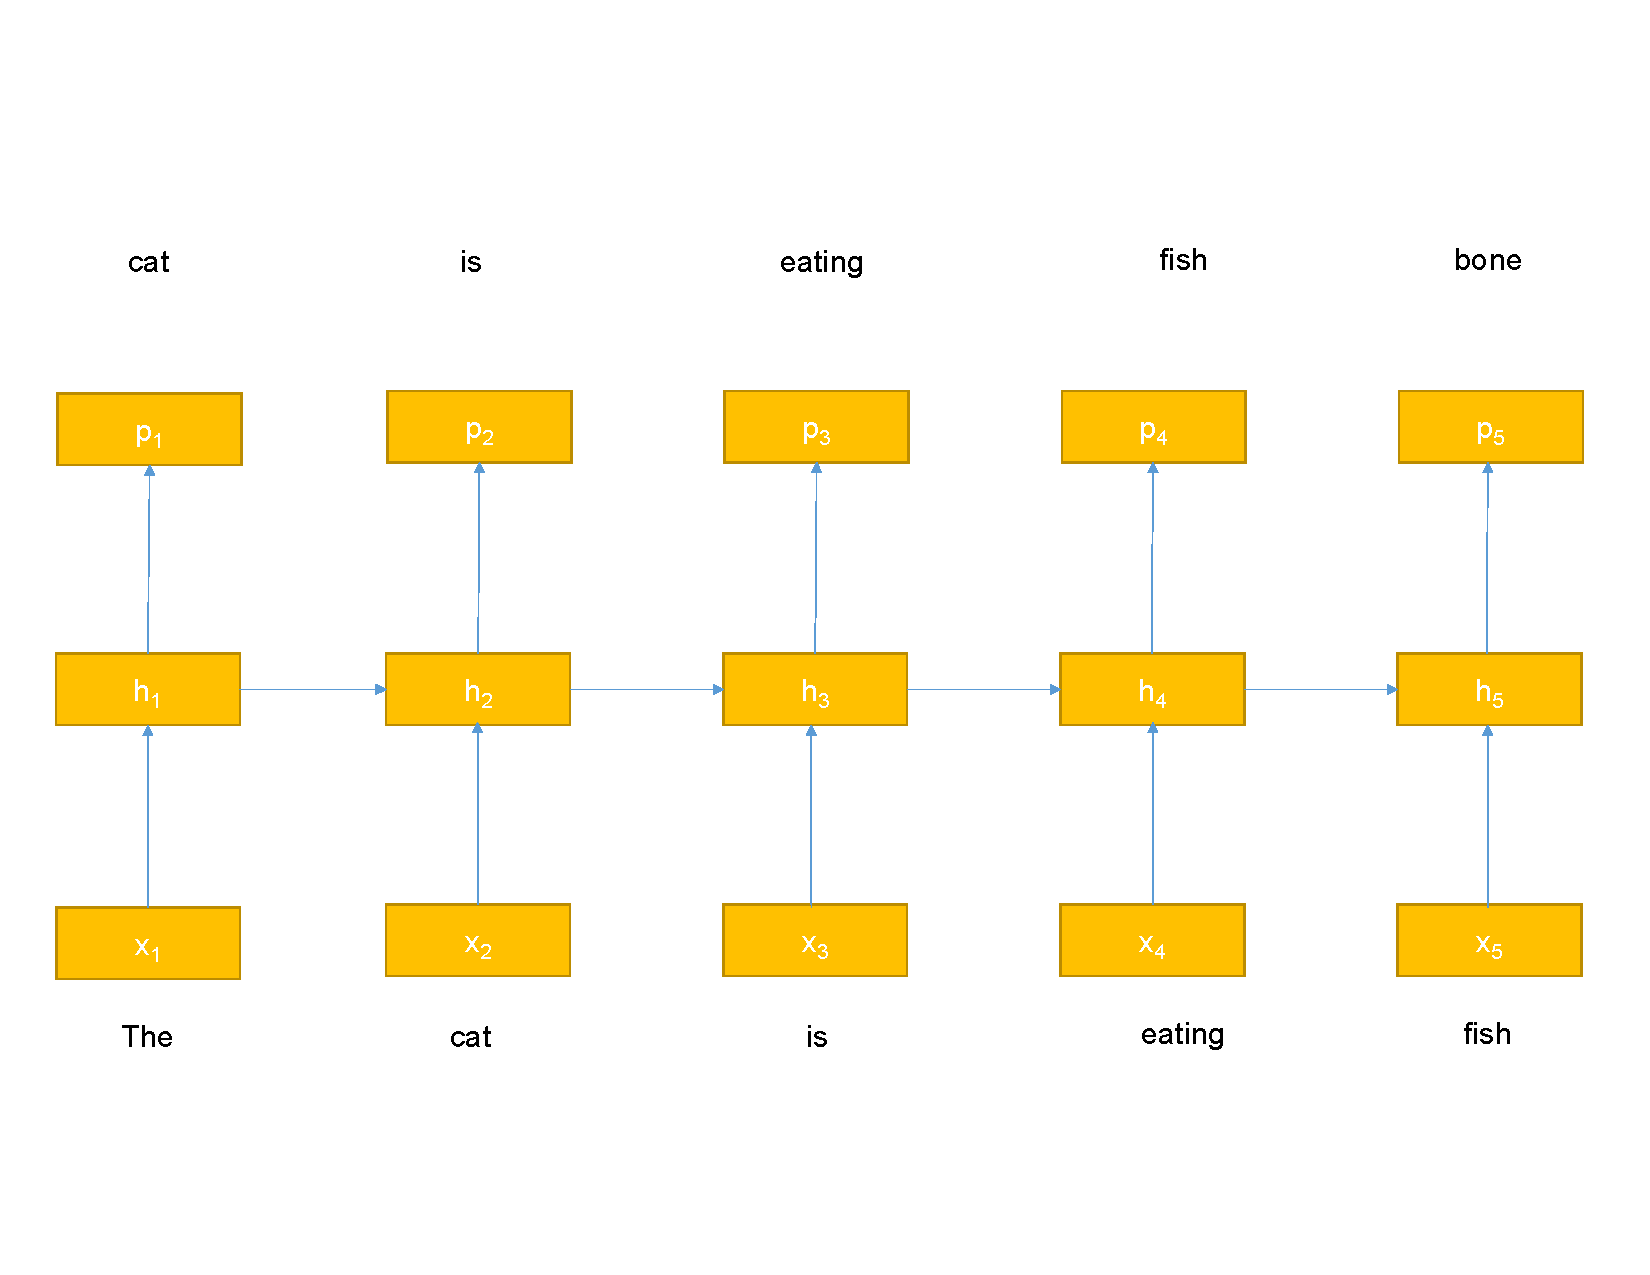
\includegraphics[width=\columnwidth]{figures/rnn.pdf}
	~ \caption{A simple RNNLM~\cite{mikolov2010recurrent} predicting the sequence ``The cat is eating fish bone''.}  
	~ \label{fig:SimpleRNN}
	~ \end{figure}


\begin{equation}
h_i = f(Wx_i +  Uh{i-1} + b)
\end{equation}

The activation function $f$ can be either Tangent Hyperbolic, Sigmoid or ReLU as mentioned before. The starting state $h_0$ is set to 0 to denote the initial state of the memory. In each time step, the RNNLM can optionally produces the probability distribution for a predicted word, given the sequence that network has scanned previously. The probability distribution over the vocabulary is derived similarly to the feed-forward networks:

\begin{equation}
\begin{aligned}
o_i = W^oh_i + b^o \\
p_i = \text{softmax}(o_i)
\end{aligned}
\end{equation}

with the Softmax function explained in Equation~\ref{eq:softmax}. To be clear, $o_i$ and $p_i$ denote the unnormalised and normalised distribution generated at time step $i$. For the language modeling scenario, the input and output samples of the network in each training iteration are two sequences $X \text{ and } Y$ in which the output sequence is the shift-by-1 version of the input sequence. The parameter set of the network including $W, b, U, W^o \text{ and } b^o$ are shared across time steps. 


\subsubsection{Training Recurrent Networks}

Similarly to the feed-forward models, The recurrent models can also be efficiently trained with stochastic gradient descent (SGD). However, since the networks contain shared parameters at arbitrary numbers of time steps, the gradients are computed differently using back-propagation through time (BPTT). The details of this algorithm are divided into two parts: the local gradients computed  at each time step, and the global gradients accumulated by un-folding the networks. 

\paragraph{At each time step}

% How to compute the gradients

\paragraph{For global derivatives}

Backpropagation through time algorithm 

\paragraph{Problems with BPTT}

Although truncated back-propagation through time provides a practical training method for RNNs, the nonlinear iterative nature of the simple RNN architecture still makes capturing long-term dependencies difficult. The two common problems encountered while training RNNs are the~\textit{exploding} and the~\textit{vanishing} gradients~\cite{bengio1994learning,pascanu2013difficulty}. On the one hand, the gradients can be exponentially large as in the back-propagation through time process which is detrimental for learning. One the other hand, we can also experience the phenomenon that gradients go quickly towards zero after being propagated through time steps. Consequently, the model is not able to track the signal and complete loses the memory trace in the past. For example, the original RNNLM normally has to truncate the BPTT at about $5-10$ steps, which has the same modeling capacity and performance with $10$-gram feed-forward models~\cite{mikolov2011extensions,hai2012measuring}. The gradient exploding problem can be tackled adequately using gradient clipping. Pascanu et al~\cite{pascanu2013difficulty} suggested to clip the norm of the gradients (for all parameters): given a gradient vector $dx$ that is computed with BPTT, if the norm $||dx||$ is greater than a threshold value $\delta$, then $dx$ would be softly scaled:

\begin{equation}
dx \leftarrow dx\frac{||dx||}{\delta}
\end{equation}

%Explain mathematically
\paragraph{Dealing with gradient vanishing}

A number of solutions were proposed to solve the gradient vanishing problem. We will make a brief review of the most prominent approaches. First, Mikolov et al~\cite{mikolov2014learning} proposed to integrate another memory layer which is formed by the bag-of-word addition of the input words over time, decays slower than the main hidden memory and is initialised as an identity matrix. The same initialisation trick is applied together with using Rectified Linear Units (ReLU) as the activation function in~\cite{le2015simple}. While both works mentioned are fairly simple, the RNNs can also be trained efficiently with second order derivatives using Hessian-Free optimization~\cite{martens2011learning}. Even though the method was prove to allow the network to acquire a reliable memory which can remain stable after hundreds of time steps, it is not easy to implement efficiently compared to traditional back-propagation. The most successful method that is applied to sequential modeling in general and language modeling in particular is the Long-Short Term Memory LSTM networks~\cite{hochreiter1997long} that use an explicit memory cell combined with a gating mechanism to intensively deal with the gradient vanishing problem.

\paragraph{LSTM Structure} The intuition of an LSTM starts from the integration of a linear memory unit, so that the gradient can flow smoothly during the back-propagation through time steps using a memory cell $c_t$. 

\begin{equation}
c_t = c_{t-1} + f(Wx_i +  Uh{i-1} + b)
h_t = c_t
\end{equation}

This approach is referred as ``Leaky integration units''~\cite{bengio2013advances}. In the BPTT process, the gradient can flow over exactly one path through the memory units $c_i$, and since $dc_i = dc_{i-1}$, the gradients are guaranteed to not vanish. The recurrent architecture should also be able to be adequately robust to train long sequences, where there are certain inputs which are irrelevant to the modeling task. Sometimes, the memory of the network should be refreshed, for example at the beginning of a new utterance in Speech Recognition~\cite{graves2005framewise} or a new sentence in Machine Translation~{sutskever2014sequence}. Hochreiter et al~\cite{hochreiter1997long} enhanced the architecture by adding flexible and trainable gates that allows the RNN to reset the memory, control the amount of input and output respectively. The adaptive gates are built from the current input $x_t$ and the previous hidden memory $h_t$. 

The gates of the network include: the forget gate $f_t$ is used to directly control the memory flow $c_t$ to cut the connection with the previous steps, the input gate $i_t$ decides the amount of input to be incorporated, the output gate $o_t$ controls the amount of memory flow to be produced for the task and finally the candidate memory unit $\tilde{C}$ that contributes to the current memory flow. All gates are defined similarly, with the first three gates use the Sigmoid activation to force the values to be in \{0, 1\}, while the candidate memory uses the Tanh activation function.

\begin{equation}
\begin{aligned}
f_t = \text{Sigmoid}(W_fx_t + U_fh_t + b_f) \\
i_t = \text{Sigmoid}(W_ix_t + U_ih_t + b_i) \\
o_t = \text{Sigmoid}(W_ox_t + U_oh_t + b_o) \\
\tilde{C}_t = \text{Sigmoid}(W_cx_t + U_ch_t + b_c) \\
\end{aligned}
\label{eq:lstm1}
\end{equation}

In the next step, we decide the new information to be stored in the new memory cell. The cell is updated by combine the input gate and the candidate memory unit. Also, the forget gate is employed to drop certain information from the previous memory cell. Consequently, we come up with a new memory cell as follows:

\begin{equation}
C_t = f_t * C{t-1} + i_t * \tilde{C}_t
\label{eq:lstm2}
\end{equation}

Finally, we update the hidden state with the new cell state and the output gate:

\begin{equation}
h_t = o_t * \text{Tanh}(C_t)
\label{eq:lstm3}
\end{equation}

In Equations~\ref{eq:lstm2} and~\ref{eq:lstm3}, the symbol $*$ denotes element wise matrix multiplication. The implementation of LSTM can be efficient by computing all gates in one single matrix multiplication, then applying the activation functions on different parts of the output. In practice, one can experience different implementation variations of LSTMs and RNNs in terms of initialisation, bias usage or different gate implementations such as the Gated Recurrent Unit~\cite{cho2014learning}. The empirical research of~\cite{zaremba2015empirical} shows that there is not any substantial difference in terms of performance between different LSTM variations. 

\paragraph{Training LSTM}

Rewrite the Backpropagation through time from RNN
%
%\section{Analysis}
%
%
%\subsection{Computational Complexity}
%
%\textbf{Bottleneck in the Softmax layer}
%
%\textbf{Approximating the Softmax}

%\section{Analysis}
%
%The most important achievement of neural network language models is the ability to model word representations with low dimension embeddings that can capture syntactic and semantic properties of words~\cite{mikolov2013distributed,mikolov2013efficient}. Such ability is trained simultaneously with the classifier in order to capture linguistic regularities, which helps the network to generalise over observed sequences. 
%
%Despite the fact that the state-of-the-art language models consist of a shared projection space between words, they still treat the context as a sequence of discrete symbols. The feed-forward network simply concatenate the word vectors and learn the non-linear mapping functions to get word combinations, while the recurrent models take one word as a time step, whose weakness is that a particular time step does not have any information about future steps. In fact, it is useful to take into account the collocations and multi-word expressions in the context. For example, the English word ``get'' can acquire different meanings when paired with different propositions, which the word embeddings hardly can represent. 
%
%Such word combinations are often identified by statistical methods~\cite{sag2002multiword}, which requires an intensive scanning through the data to find frequent combinations. In the context of the neural networks, it is intuitive to use a special neural network layer that has the~\textit{convolution} property, which goes through the input sequence by scanning with a small window to find pattern features. 





%~ \chapter{``Copy'' Mechanisms}
%~ \label{c:copy}

%~ \chapter{Attention Mechanisms}
%~ \label{c:attention}
%~ \input{4-attention.tex}

%~ \chapter{Hybrid Neural Machine Translation}
%~ \label{c:hybrid}
%~ \input{5-hybrid.tex}

%~ \chapter{Towards the Future of NMT}
%~ \label{c:future}
%~ \input{6-future.tex}

%~ \chapter{Conclusion}
%~ \label{c:conclude}
%~ \input{7-conclude.tex}


% -- Appendix --
\appendix
\chapter{Publications by Author}
%\begin{thebibliography}{1}
%    \bibitem{fo} Bob Tadashi Wakabayashi {\em Anti-Foreignism and Western
%    Learning in Early-Modern Japan} 1986: Harvard University Press.
%\end{thebibliography}
\begin{itemize}
	
	\item 2016 
	\begin{itemize}
		\item 
	\end{itemize}
	
	\item 2015
	\begin{itemize}
		\item 
		
		\item 
	\end{itemize}
	
\end{itemize}

\bibliographystyle{plainnat}
\bibliography{thesis}
\end{document}
